\chapter{Integration of Transcriptomic with Proteomic data}\label{ch:Integration}
After assessing the similarity of the human gene expression profiles
across various tissues
at transcriptomic level (with \Rnaseq\ studies in \Cref{ch:Transcriptomics})
and proteomic level (with \emph{bottom-up} \ms\ studies in \Cref{ch:proteomics}),
my next step is to examine how these gene expression profiles
compare between these two different biological layers.

I have performed the integration and all the analyses presented in this chapter
under the supervision of \alvis\ and \jyoti.
A manuscript describing this work
and the new method of protein quantification, presented in \Cref{sec:NewQuantProt},
is being prepared.

A few closely related studies~\mycite{SciRep2016,Franks2017-bp} have
been published while I was working on
the integration of the non-diseased human transcriptome and proteome.
As their analyses rely on the same data sets (\ie\ \uhlen, \gtex, \pandey\ data)
that I include in my work,
I describe and discuss together my results and theirs
whenever relevant.

\derivativeWork{}
\begin{itemize}[topsep=0pt,nosep]
    \item (poster) CSHL  Biology of Genomes 2015 --- A feasibility study:
        Integration of independent human \Rnaseq\ and proteomic datasets
\end{itemize}

\clearpage\

\vspace{-1cm}

One on-going debate in the literature is
whether good correlations of expression levels should prevail or not
between matching \mRNAs\ and proteins \mycite{Uhlen:2016}.
The implicit assumption of a proportional relationship is persisting
because of the many remaining technological limitations \mycite{Vogel2012-sq},
whereas to date, the existence of a given \mRNA\ transcript or its concentration
are usually insufficient to ensure detection of the protein in a sample.

On the one hand,
\citet{Ramakrishnan2009-lv} report that
\mRNAs\ abundance are roughly sufficient to predict
the protein presence or absence from a sample and
\citet{Vogel2010-ux} that
\mRNA\ level estimations and sequence features are enough to predict
two-thirds of the human protein abundance variation.

On the other hand,
there is a lack of high correlations
between the transcriptome and proteome
(for any organism) observation in the literature.
Previous investigations found low or no correlation
between the observed expression profiles of the \mRNAs\ and
proteins~\mycite{Anderson1997-le,Chen2002-ob,Tian2004-hh,Pascal2008-gh,%
Gry2009-zv,Lundberg2010-gk}.
This observation lack is unrestricted to human \mycite{Ghazalpour2011-nb} or
even mammals~\mycite{Gygi1999-fl,Maier2009-pb,Maier2011-tz,Yeung2011-sl,%
Palmblad2013-ji,Freiberg2016-fu}.

Additionally,
Schwanhäusser et al.~\mycite{schwanhausserglobal:2011,Schwanhausser2013-et}
present rather moderate correlations ($r^2≤0.41,\ie~r<0.64$)
for their encompassing experiment
and highlight that \mRNAs\ levels explain only about 40\% of protein variations
they have observed.

Other studies tried to explore the \mRNAs\ and proteins relationship in answer
to stimuli.
\citet{Marguerat2012-sn} report for yeast that
steady-state cells present an equivalent level of correlation ($r^2=0.36,
\ie~r=0.6$) to the previous studies,
while proliferating cells present higher correlations ($r^2=0.55, \ie~r=0.74$).
\citet{Jovanovic2015-wv} identify \mRNA\ fold changes
as the most prominent contributor to the relative changes in protein expression
for 89\% of the mouse immune genes of their study,
before concluding that relative changes in \mRNAs\ levels can explain
\emph{relative} changes in protein levels,
while post-transcriptional regulations (including degradation rates)
better explain the \emph{absolute} amount of proteins.

While many other regulations processes may occur,
post-transcriptional modifications and technical noise
are (still) perceived as the probable primary sources
of \mRNA/protein concentration discrepancies~\mycite{Vogel2012-sq,Plotkin2010-ug}.
Although
the joint study of transcriptome and proteome has already helped to highlight
links between genotype and phenotype~\mycite{Vogel2012-sq},
the previous mitigated results probably explain the focus shift of
many subsequent studies.
Previous efforts were about linking the actual expression levels.
More recent studies primarily compare qualitative attributes
of given proteins and related \mRNAs,
such as their presence or absence in a specific condition
or tissue~\mycite{Santos2015-rj,Freiberg2016-fu,Uhlen2015}
or their differential expression profiles across the same set of conditions
to detect any discrepancy~\mycite{Varemo2015-uk}.

All (or almost all) aforementioned studies have all turned to cells
for their joint analyses of transcriptome and proteome.
The analyses and integration I present in this chapter are,
on the contrary, based on tissue studies.

\vspace{-2mm}
\section{Data~and~principal~analytical~approaches}\label{sec:IntegrationData}
\vspace{-4mm}
Since 2014 and the human proteome drafts \mycite{PandeyData,KusterData},
this is the first time with such
an unparalleled availability of large-scale tissue studies
both at the transcriptomic and proteomic layers to explore and integrate together
(see \Cref{ch:datasets}).
While these data are independent
(collected from various individuals, prepared,
and characterised by different laboratories),
their combined study may help
to shed light on the relationship
between the transcriptome and proteome at the tissue level.
Using different sources for the transcriptome and proteome
increases the overall technical noise,
but it may also help to highlight relevant biological signals (as
they need to be stronger than the noise and batch effects to be captured).

In \Cref{ch:Transcriptomics}, I show that
the transcriptome \Rnaseq\ datasets present high correlations
(median value for Pearson: $r_{\setOneMath}=0.75$; $r_{\setTwoMath}=0.85$ ---
Spearman: $\rho_{\setOneMath}=0.88$; $\rho_{\setTwoMath}=0.93$).
For this chapter analyses,
I only consider the datasets with the highest similarity
(highest correlations) and
that incidentally comprise the greatest number of tissues
and are the two most recent studies,
\ie\ \dataset{Uhlén \etal}~\mycite{Uhlen2015}
and \dataset{Gtex}~\mycite{GTExTranscript} data.

Since I am reusing published data,
the initial experimental designs are suboptimal for my study.
Using both \uhlen\ and \gtex\ data
allows filtering out \mRNAs\ with high variability.
Whether this variability is technical or biological is irrelevant;
in both cases,
interpreting the relationship
between a highly variable \mRNAs\ and its protein from another dataset
remains hard to interpret.
Besides, the comparison of the two transcriptomic data creates a reference,
\ie\ an ideal scenario.

On the other hand,
the technical variability prevails over
the biological signal of same-tissue samples
for the available high-throughput proteomics,
as shown in \Cref{subsec:protTechVarHigh}.
To avoid an overly restricted protein set for the following analyses,
I only include one proteomic study: \pandey\ et al.~\mycite{PandeyData}.
All its samples have been run through the same \ms\ platform and
with the same protocol.
Besides, it presents more homogeneous protein distributions
(see \Cref{fig:distribProt} and \Cref{fig:pandeyDistribQ1Q2}) and
quantifies more proteins per tissues (\Cref{fig:distribProtUniq3D})
than the two other datasets.
As one of the main current limitations of bottom-up \ms\ proteomic studies
is the possible lack of detection of proteins for various reasons
(see \Cref{subsec:simpleProt}),
it suggests that
the \pandey\ data has a higher quality than the two other datasets.

%Many strategies are recommended to increase the depth of the coverage
%(\eg\ \mycite{Zhang2014,Eriksson2007-si,Koziol2013-si}).
%Put together these facts suggest that
%the \pandey\ data has a higher quality than the two other datasets.
\vspace{-0.5mm}
Finally, the literature reports that
the proteome is more conserved than the transcriptome
(across individuals and species)~\mycite{Laurent2010-rg,Liu2016-re}.
Hence, this data collection ought to provide a crude estimate
on the extent of observations that hold from cell to tissue level.

This chapter integration and analyses are based on the common set of tissues
and matching pairs of \mRNA/proteins.

\vspace{-2.5mm}
\subsection{Overlapping set of tissues for the three datasets}

\begin{figure}[!htbp]
    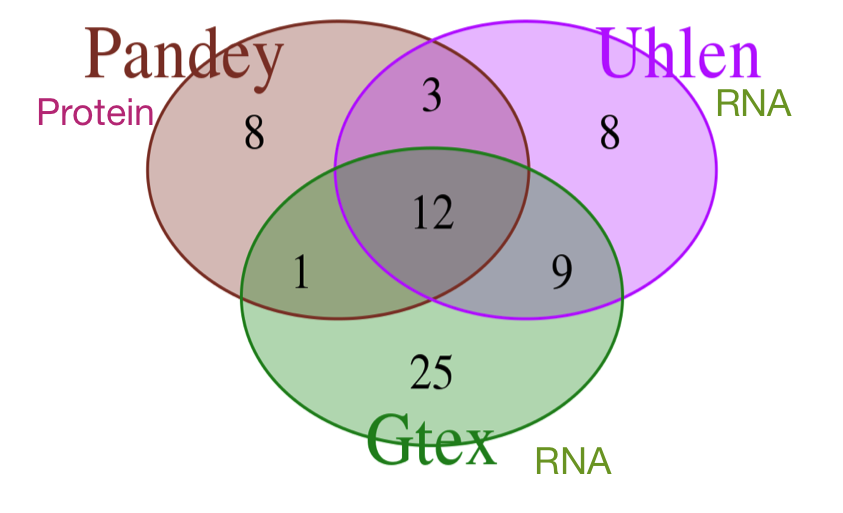
\includegraphics[scale=0.61]{integration/PandeyGtexUhlen_tissuesVenn.pdf}
    \centering
    \vspace{-5mm}
    \caption[Number of share and unique tissues between the proteomic
    dataset from Pandey \etal\ and the transcriptomic datasets (Uhlén \etal\ and
    Gtex)]{\label{fig:VennTissuePandeyGtexUhlen}\textbf{Number of share and unique
    tissues between the proteomic (Pandey \etal) and the
    transcriptomic (Uhlén \etal\ and GTEx) data.} The twelve common tissues of
    the three datasets are:
    \tissue{Adrenal gland}, \tissue{Bladder}, \tissue{Colon}, \tissue{Oesophagus},
    \tissue{Heart}, \tissue{Kidney}, \tissue{Liver}, \tissue{Lung}, \tissue{Ovary},
    \tissue{Pancreas}, \tissue{Prostate} and \tissue{Testis}. The three added
    tissue between \dataset{Uhlén \etal} and \dataset{Pandey \etal} are:
    \tissue{Gall bladder}, \tissue{Placenta} and \tissue{Rectum}. The added tissue
    between \dataset{GTEx} and \dataset{Pandey \etal} is the \tissue{Frontal
    cortex}.}
\end{figure}

All the analyses are including the twelve shared tissues between the three
datasets (\adrenal, \Bladder{}\footnote{May also
be referred as \tissue{Urinary Bladder}},
\hColon, \Oesophagus, \Heart,
\Kidney, \Liver, \Lung, \Ovary, \Pancreas,
\Prostate\ and \Testis).

\vspace{-1.5mm}
In a few cases, I have also extended the analyses by excluding the \gtex\ data
to include the three added tissues shared by
\pandey\ et al.\ and \uhlen\ et al.\ data (\ie\ \Gall, \Placenta\ and \Rectum).

\vspace{-2mm}
\subsection{Matching pairs of mRNAs and proteins}

\vspace{-3mm}
As formerly described in \Cref{sec:bias_sources},
to avoid unnecessary biases I only consider for the following analyses
\mRNAs\ (\ie\ \glspl{RNA} with a \emph{protein-coding} biotype --- \ens{76})
and proteins that are found in each dataset at least in one of the included tissues.

Besides, while there is only one value per protein per tissue,
both \uhlen\ \etal\ and \gtex\ data present replicates,
\ie\ there are several values per \mRNA\ per tissue
for each of the transcriptomic datasets.
Thus, I use the \enquote{virtual references},
\ie\ \treps\footnote{\glsdesc{TREP}}
that I describe in \Cref{subsec:averagedTissue},
to avoid unbalancing the analyses.

\begin{figure}[!htpb]
    \includegraphics[scale=0.65]{integration/PandeyGtexUhlen_mRNAprotQ1Venn.pdf}\centering
    \vspace{-5mm}
    \caption[Distribution of the unique and shared proteins/mRNAs for the three datasets
    across twelve tissues]{%
    \label{fig:PGU_vennQ1}\textbf{Distribution of the unique and shared proteins
    of Pandey et al.\ data and \mRNAs\ from Uhlén et al.\ and GTEx ones across
    their twelve shared tissues.}
    There are 6,357 matching gene products between the three datasets.
    Only 5 proteins have apparently no matching partners
    in the \uhlen\ \etal\ or \gtex\ data.}
\end{figure}

\Cref{fig:PGU_vennQ1} presents the proteins from the \pandey\ \etal\ data
quantified through the pipeline described in \Cref{subsec:msDataProcess}
and the \mRNAs\ of \uhlen\ \etal\ and \gtex\ data quantified by \htseq\
(see \Cref{subsubsec:RnaseqDataProc}).
Almost all proteins are matching to a \mRNA{}.
\Cref{fig:PU_vennQ1} is the same analysis and result
with the three added tissues shared solely by \pandey\ \etal\ et \uhlen\ \etal\ data
and without the \gtex\ data.

\begin{figure}[!htpb]
    \includegraphics[scale=0.65]{integration/PandeyUhlen_mRNAprotQ1Venn.pdf}\centering
    \vspace{-5mm}
    \caption[Distribution of the unique and shared proteins/mRNAs for Pandey et al.\
    and Uhlén et al.\ across fifteen tissues.]{%
    \label{fig:PU_vennQ1}\textbf{Distribution of the unique and shared proteins/mRNAs
    for Pandey et al.\ and Uhlén et al.\ across their fifteen shared tissues.}
    The number of matching pairs (6,428) and proteins that lack a counterpart in
    the transcriptomic data (8) are similar regardless on how many different
    transcriptomic data is included (see \Cref{fig:PGU_vennQ1}).}
\end{figure}

As shown in \Cref{fig:PGU_vennQ1,fig:PU_vennQ1},
only about 32\% of the quantified \mRNAs\ in the \uhlen\ \etal\ and \gtex\ data
have a corresponding proteins in the \pandey\ \etal\ data.
The protein quantification (provided by \james) follows
a state-of-the-art protocol and very stringent parameters.
Accurate protein quantification is paramount for reliable proteome exploration.
However, since my aim is to integrate proteomic data with transcriptomics,
more flexible protein identification and quantification are possible.

The new quantification that I devised for the purpose of this chapter analyses
was implemented by \james.
As described in \Cref{sec:NewQuantProt},
it is based on an \Rnaseq\ quantification approach and
takes advantage of the \emph{degenerate} peptides
to allow the quantification of proteins
even if they only have two unique peptides.

\begin{figure}[!htbp]
    \includegraphics[scale=0.68]{integration/PandeyGtexUhlen_mRNAprotQ3Venn.pdf}\centering
    \caption[Distribution of the unique and shared proteins/mRNAs
    across the three datasets and twelve tissues
    (with the new protein quantification method)]{\label{fig:PGU_venQ3}%
    \textbf{Distribution of the unique and shared proteins/mRNAs
    across the Pandey et al.\ (processed with the new quantification method),
    Uhlén et al.\ and GTEx data across their twelve shared tissues}.
    }
\end{figure}

\begin{figure}[!htbp]
    \includegraphics[scale=0.68]{integration/PandeyUhlen_mRNAprotQ3Venn.pdf}\centering
    \caption[Distribution of the unique and shared proteins/mRNAs for the
    Pandey et al.\ (processed with the new quantification method) and Uhlén et al.\ data
    across the fifteen tissues.
    ]{\label{fig:PU_vennQ3}\textbf{Distribution of the
    unique and shared proteins/mRNAs} for
    the Pandey et al.\ (processed with the new quantification method)
    and Uhlén et al.\ data across the fifteen tissues.}
\end{figure}

\Cref{fig:PGU_venQ3,fig:PU_vennQ3} are
the counterparts of \Cref{fig:PGU_vennQ1,fig:PU_vennQ1}.
With the new quantification method for the \pandey\ \etal\ data,
about 62\% of the \mRNAs\ quantified in the \uhlen\ \etal\ and \gtex\ data
are matched to a protein.

After comparing the respective lists of \emph{undefined} (see \Cref{sec:ExpressedOrNot})
proteins and \mRNAs\ (between \dataset{Pandey \etal} and \dataset{Uhlén \etal} data and
between \dataset{Pandey \etal} and \dataset{Gtex}),
I have excluded these unmatched proteins and \mRNAs\ from the following analyses
which only include the matching \emph{defined} proteins and \mRNAs\ triplets
(or pairs depending on the inclusion of the \gtex\ data).
The lists of proteins lacking a matching \mRNAs\ in \ens{76} is provided
in \Cref{tab:protNoTrans}.

Since the results are similar regardless of the quantification used
for the proteomic or transcriptomic data,
the reported figures in this chapter are using
the second more extensive set of proteins.
For some analyses,
figures based on the first protein quantification method
are also provided as supplementary data.
Note that there may be differences for individual genes.

Finally, as in \Cref{ch:Transcriptomics},
all the proteins and \mRNAs\ from the mitochondrial genome are removed
from further analyses
(see \Cref{subsec:mito}).

\subsection{Tissue-centric and gene-centric analyses}

\Cref{fig:visualexp} summarises the two analytical approaches I use
to compare transcriptomic and proteomic data.
In fact,
\citet{Liu2016-re} emphasise how important it is to clearly define
the approach when reporting results to avoid many confusions.
The \emph{tissue-centric} approach compares for each tissue
the global expression of its transcriptomic landscape to its proteomic one.
In contrast,
the \emph{gene-centric} approach compares for each gene
the expression levels of its \mRNA\ to its protein ones across all the tissues.

\begin{figure}[!htpb]
    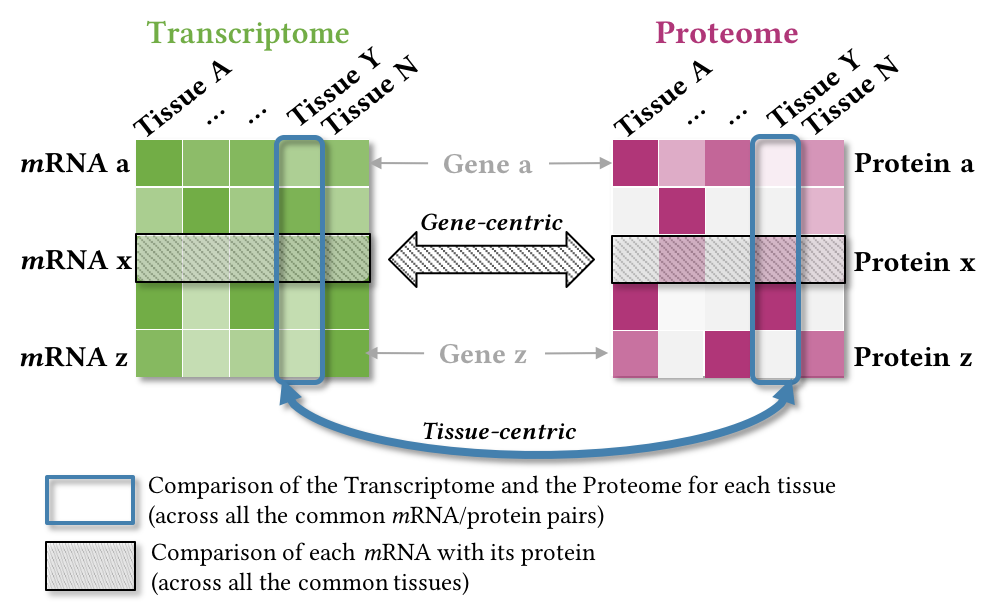
\includegraphics[scale=0.75]{integration/VisualExplaination-Lin.png}\centering
    \caption[Summary of the expression comparison approaches between
    the transcriptome and proteome]{\label{fig:visualexp}\textbf{Approaches
    summary of the expression comparison between the transcriptome and proteome.}
    \emph{Tissue-centric} analyses focus on
    how the transcriptome and proteome relate to each other within the same tissue.
    \emph{Gene-centric} analyses study for each gene how its \mRNA\ expression
    levels across all (or a subset of) the tissues may relate to
    the quantified expression levels of its corresponding protein.
    }
\end{figure}


\section{Results}\label{sec:IntegrationResults}


We attempt to found out if the lesser correlations reported at cell levels would
hold at tissue level.
Our findings are actually supporting the first assumption; there is a good correlation
between the transcriptomic and proteomic data, even though all the samples used in
the study are all completely independent. Moreover, there is a high consistency
between tissue-specific proteins and tissues-specific genes.

In fact, here, even though I have only access to independent data,
the average Pearson correlation per tissue is above $0.5$
$[$min: $0.45$ (\Oesophagus); max: $0.666$ (\Liver)$]$.

%%%%%%



Present that we develop a new method of quantification:
increase the number of proteins that are identified and quantified per tissues.
For each analyses: one result with the conservative quantification
and another one with the new quantification.

%\subsection{New quantification method for the proteomic data}\label{subsec:IntegrationNewMethQuant}


In the context of this work (\ie\ when focusing on the 15 common tissues between
the \dataset{Uhlén \etal} and the \dataset{Pandey \etal} datasets),
he has quantified about 6,400 proteins with
the standard method. With the new approach, he has quantified a more substantial set of
proteins: about 12,300 proteins. This new number is quite close to the initially
reported number of protein by Kim \etal\ study.
Indeed the original paper is describing proteins encoded by 17,294 genes.

Moreover, all tissues and cell lines are evenly impacted
(\ie\ none of them is dramatically affected compared to the others).

As shown in~\cref{fig:VennGeneTransProt15}, there are 14,617 pairs of
proteins/genes.
We expect a greater number of transcripts than proteins \TK{add references}.
Thus, it may be primarily surprising that
few proteins lack a match in the transcriptome data
(see supplementary Table~\cref{tab:protNoTrans}).
There are several possible explanations.
\begin{itemize}[topsep=0pt,nosep]
\item It may be a technical issue or an artefact on the transcriptomic side.
    \begin{itemize}[topsep=0pt,nosep]
        \item \mRNAs\ are present but the capture missed them at the library preparation
        step (see \cref{subsec:libPrep}) for a reason or another.
        \item Mapping algorithms have misassigned reads of
        \mRNAs\ with a high sequence-similarity to others.
        \item The annotation lacks \mRNAs\ definitions.
    \end{itemize}
\item It might also be that the protein doesn't belong to the sample: the identification
is a false positive or incorrect; the sample\footnote{Or the instrument used for
the capture} might also have been contaminated at some point with some foreign
proteins.
\item It can also be due to an underlying biological phenomenon:
the turnover of the \mRNA\ is very low, while the protein is very stable;
the proteins have been expressed somewhere else and then has been imported in the
current tissue (\eg\ hormones or cytokines). Finally, as the proteome
and transcriptome used for this study have been collected independently, if the
gene is individual- or population-specific, we will then detected in one of the
study and not in the other one. However, as we have biological replicates on the
transcriptomic side, this last hypothesis seems the most unlikely.
Of course, a mixture of the previous causes is also highly probable.
\end{itemize}

\begin{figure}[!htbp]
    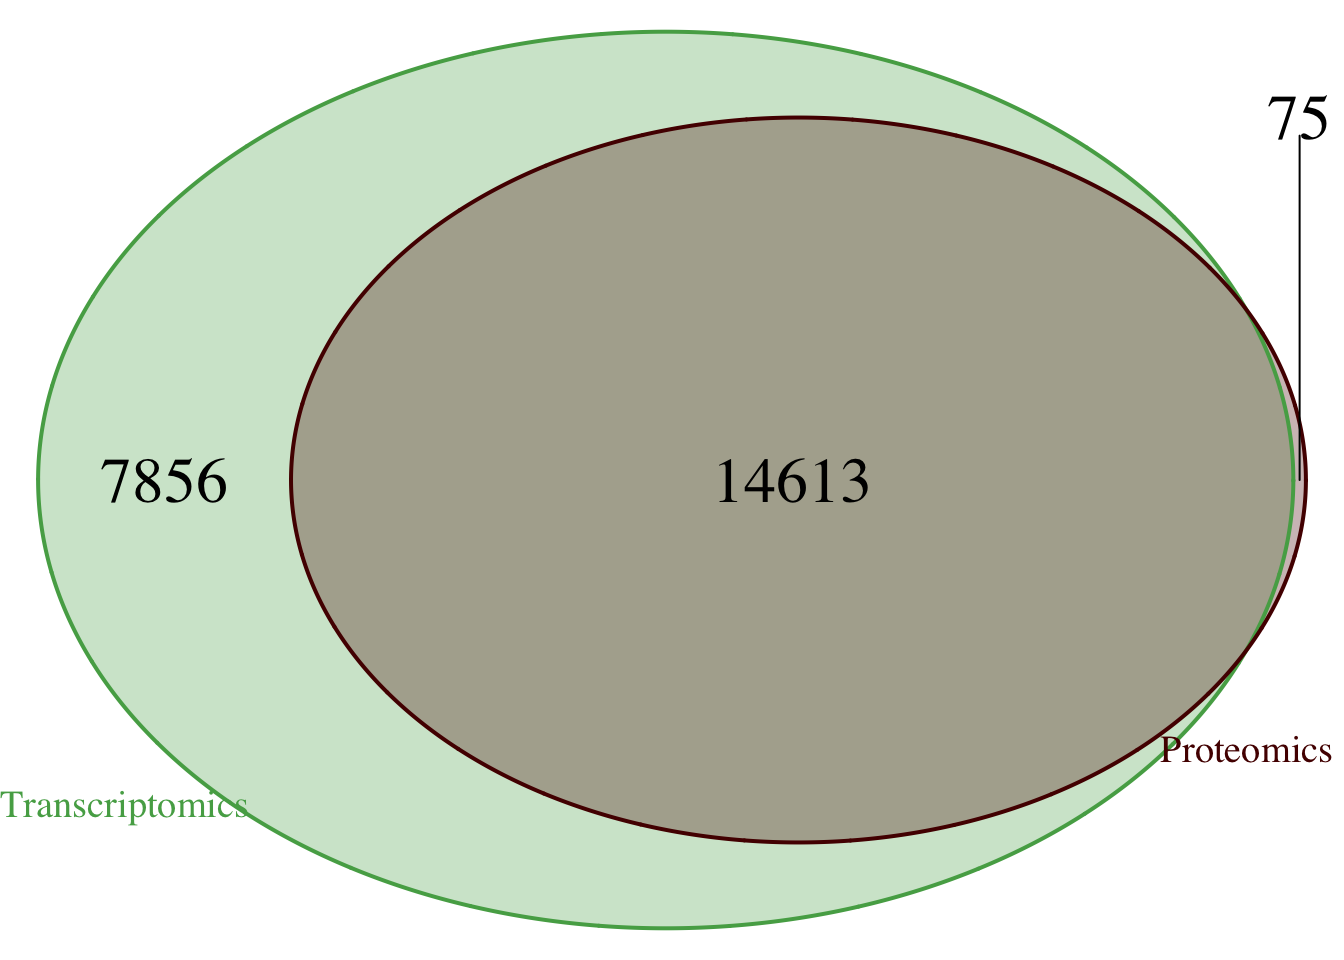
\includegraphics[scale=0.15]{integration/VennGeneTransProt15}\centering
    \caption[Unique and shared protein/gene pairs between Proteomics
    (Pandey \etal\ (PPKM)) and
    Transcriptomics (Uhlén \etal\ (\gls{FPKM}))]
    {\label{fig:VennGeneTransProt15}\textbf{Unique and shared protein/gene
    pairs between Proteomics (Pandey \etal\ (PPKM)) and Transcriptomics (Uhlén
    \etal\  (\gls{FPKM})).} There are 14,613 pairs common between the
    transcriptomic (only the protein coding genes are considered)
    and the proteomic dataset.}
\end{figure}

I have performed the analyses presented in this chapter on both sets of
quantification. As the high-level results and conclusions are remaining the same,
the figures and discussions hereafter are based on
the new quantification method. For comparison purposes,
I have produced (following the same analyses and with their associated
implementations) some figures and tables from the data quantified by the first
method. Those can be found in the appendices; their references
are given in blue (and in brackets) in the caption of the main figures.

In the following sections, we consider the proteomic data with this new
quantification method and compare it to the \dataset{Uhlén \etal} dataset
for their 15 common tissues.

\subsection{Expression profile of proteomics and transcriptomics look very
similar in shape on a logarithmic scale}
\label{subsec:IntegrationExpProfileSim}

As discussed in the previous chapters, visualising the data is very important
prior to any computation. It allows to detect if we are violating
any assumption or if there is any issue with the data. In fact, we have seen
in~\cref{ch:Transcriptomics} that there is an issue with the pancreatic
samples for the \dataset{Uhlén \etal}, as the range of genes expression is quite
different from the other samples/tissues.

Considering the scale of expression between the proteomic assay and the
transcriptomic ones, they are not directly comparable. Hence,
all the data (regardless of the method of quantification) have been transformed
with $X_{i}=\log_{2} (x_{i}+1)$ (or $X_{i}=\log_{2} (x_{i})$)
before any other computation or visualisation.


\begin{figure}[!htbp]
    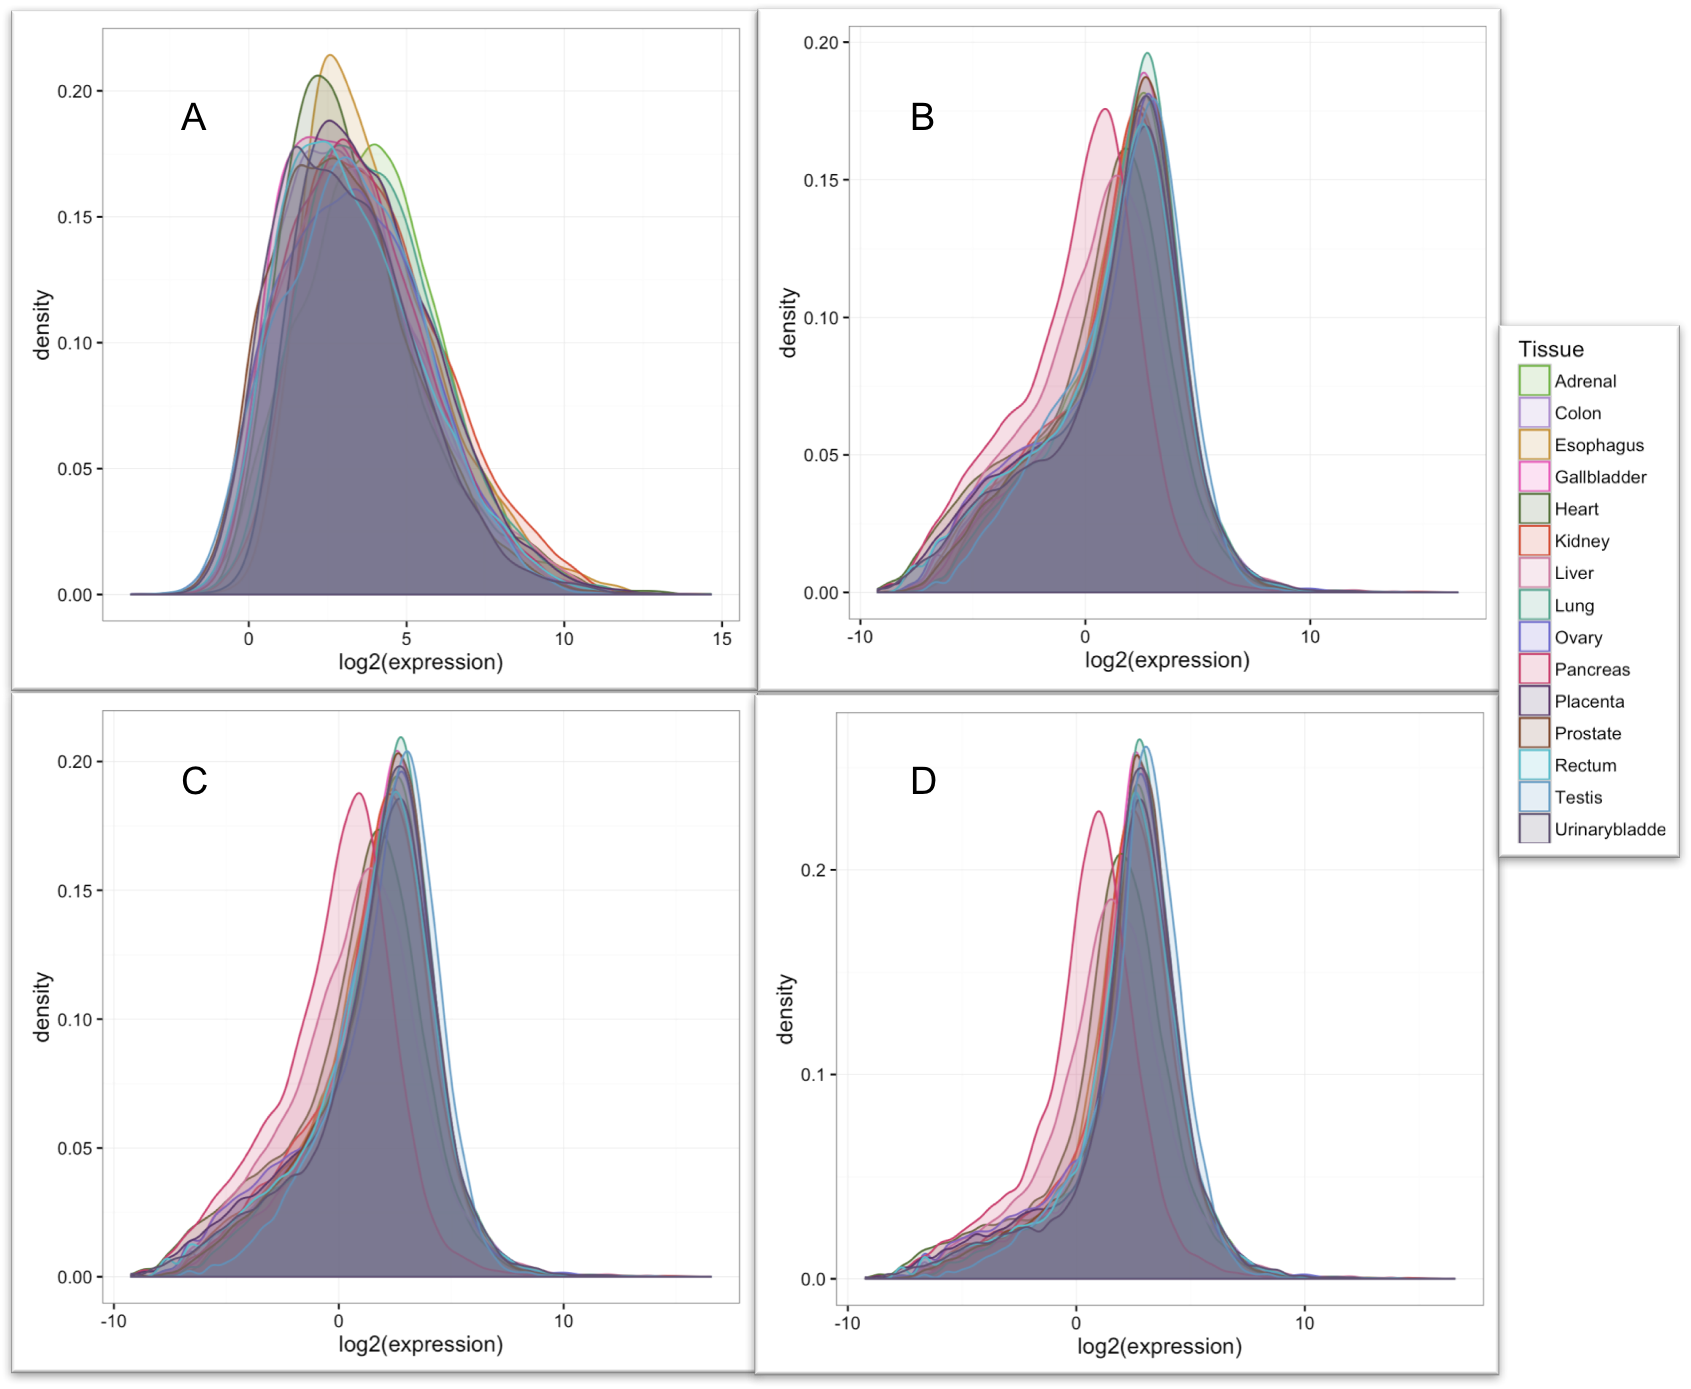
\includegraphics[scale=0.45]{integration/densityExpProtTrans15}\centering
    \caption[Density of expression of proteins and \mRNAs\ per
    tissues.]
    {\label{fig:densityExpProtTrans15}\textbf{Density of expression of
    proteins and \mRNAs\ per tissues.} \\\textbf{A}| Proteins.
    \textbf{B},\textbf{C},\textbf{D} present the same data but with
    different thresholds:
    \textbf{B}| No threshold. \textbf{C}| 1 \gls{FPKM}.
    \textbf{D}| 5 \glspl{FPKM}.\\The threshold used for the proteins is the
    threshold of
    detection (\ie\ greater than zero). The different density of distributions are
    globally gaussian. When the threshold is increased for the transcriptome, the
    shape get closer to the ideal one, as the bulge created by lowly expressed
    genes is removed. We can also observe that the problem with the pancreatic
    tissue get more highlighted with higher thresholds.}
\end{figure}

\Cref{fig:densityExpProtTrans15} presents the density of expression
of proteins and \mRNAs\ per tissue. In~\cref{fig:densityExpProtTrans15}|A,
we notice that the densities of expression of the proteins have a similar gaussian
shape for each of the tissues. We can also observe than the expression values
of the proteins gather towards the very low values.
In~\cref{fig:densityExpProtTrans15}|B to~\cref{fig:densityExpProtTrans15}|D,
we can observe the density of expression values for
the \mRNAs\ across all the tissues for
different threshold cut-off: $0$, $1$ and $5$ \glspl{FPKM}.
We remark that when we increase the threshold, the shape
of the density becomes closer to a lorentzian.~\Cref{fig:densityExpProtTrans15}|B
displays the density of expression for \emph{any} detected \mRNA\@. We can
then observe a bulge composed by the very lowly expressed \mRNAs\, for which it
is hard to decipher which are the one that are translated into proteins and which
should be considered as translational noise. When I use $1$ \gls{FPKM} as a threshold,
we observe density curves that are closer to the ideal one and these \mRNAs\ are
more likely translated into proteins.

\TK{NEED TRANSITION to comparison tissue levels for the two layers!}

\subsection{Independently human sourced transcriptomics and proteomics
have good and significant correlation for same-tissue pairs.}
\label{subsec:IntegrationGoodCorrProtTrans}

I used the whole set of common expressed \mRNAs\ and
expressed proteins\footnote{Without any other constraint: \eg\ the \mRNA\ and
its corresponding protein do not have to be detected in the same tissue.}.
Then, I calculated the correlation between the proteome and the trancriptome for
each tissue, \ie\ for each tissue, I compared each protein expression value to
its corresponding gene one.

As I exposed in~\Cref{ch:Transcriptomics}, there are some
\mRNAs\ that are lowly or even anti-correlated between the different
transcriptomic datasets.
As I can not pinpoint whether this is due to \emph{biological} or \emph{technical}
reasons, we choose to exclude the anticorrelated \mRNAs\ between \dataset{Uhlén
\etal} and \dataset{Gtex} (across the 23 common tissues) as these two datasets have
very similar protocols and have been sequenced on similar sequencers (Illumina
HiSeq 2000/2500).

As illustrated in the supplementary~\cref{fig:ScatterPlotLiver}
and~\cref{fig:ScatterPlotOesophagus}, while the exclusions of these genes might
slightly improve some of the results, it can also have a feeble opposite effect
in some other cases.
Indeed, some pairs of \mRNA/protein might have a very tight relationship in some
tissues and looser in others. Whilst this could be due to technical reasons, it
could also be due to biological ones. Unfortunately, with our current knowledge
of the datasets, it is not possible to reject pairs \emph{a priori}.

In this context, the range of Pearson correlation coefficients between the
proteomic and the transcriptomic data is from $0.66$ for the \tissue{Liver}
to $0.46$ for the \tissue{Oesophagus}.\footnote{\textbf{NB}: If I exclude the
pairs where the \mRNA\ is expressed below $1$ \gls{FPKM}, the Pearson correlation
coefficients for each tissue are substantially identical.}

\begin{figure}[!htbp]
    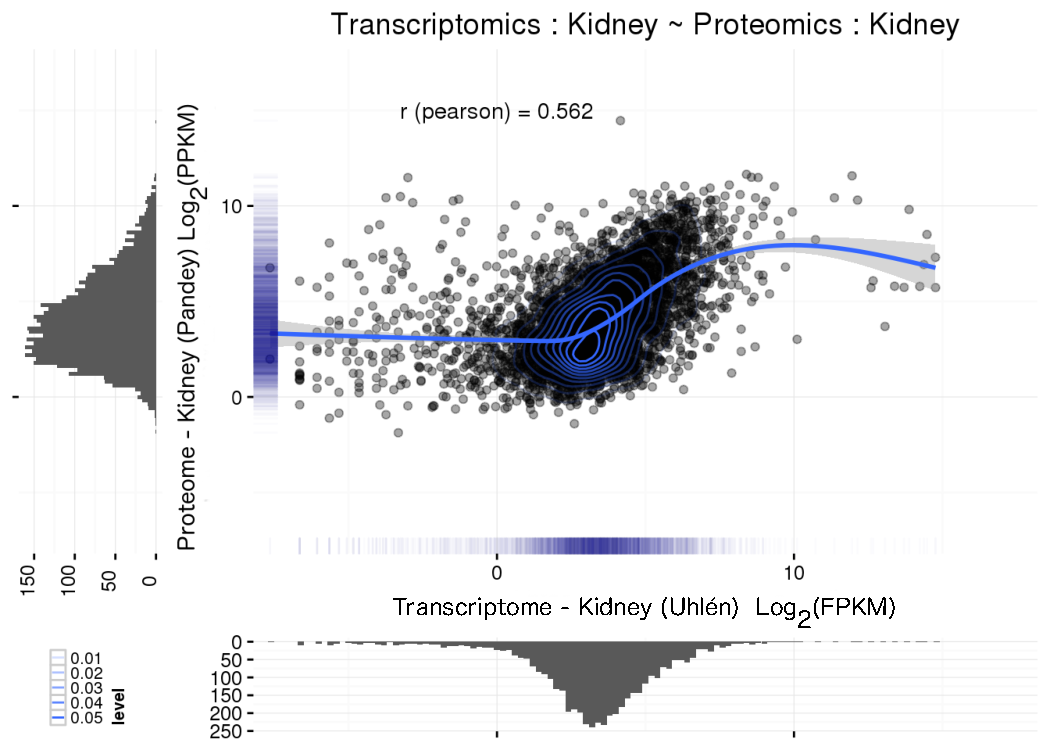
\includegraphics[scale=0.85]{integration/Kidney_scattplot.pdf}\centering
    \caption[Scatter plot of the expression value of the proteins (Pandey)
    and the \mRNAs\ (Uhlén \etal) for Kidney]
    {\label{fig:ScatKid}\textbf{Scatter plot of the expression value of the
    proteins (Pandey) and the \mRNAs\ (Uhlén \etal) for Kidney.}
    This scatter plot displays the
    log-transformed ($Log_{2}$) expression value of
    each \mRNA\ on the x-axis and the log-transformed ($Log_{2}$)
    expression value of the proteins on the
    y-axis. Each point represents a corresponding pair of \mRNA\ and protein.
    We can notice that most of the \mRNA/protein pairs are very close to
    the diagonal, which indicates a high correlation between the level
    of \mRNAs\ and proteins. We also see that the lower levels of expression of
    \mRNAs\ are more prone to the dispersion ($<0$ on $Log_{2}$-scale, so $<1$
    \gls{FPKM} on the original scale, which is a common threshold used for the
    coding \mRNAs). Besides, the proteins present most-likely a
    saturation effect of their expression values. The highest expressed protein
    is \protein{\gls{HBB}}
    (\ie\ Hemoglobin Subunit Beta) which is also found in the 5 highest
    expressed proteins in all the other tissues. It is quite likely that for
    most of the tissues, this is due to how they have been sampled.
    \\The distributions of the proteins and the \mRNAs, plotted on the outer part
    the figure, have similar shaped.\\
    \textbf{N.B.:} Whilst every pair of \mRNA\ and protein has been used to
    calculate the correlation, the pairs with a null element have been not plotted
    to optimise the visualisation.}
\end{figure}

\Cref{fig:ScatKid} illustrates the comparison of the proteomic data to the
transcriptomic data for the \tissue{Kidney} which stands within the middle of the
correlation range as its coefficient is equal to $0.56$.
The x-axis represents the level of the \mRNAs\
expression on a $Log_{2}$-scale and the y-axis represents the levels for the
proteins (also on a $Log_{2}$-scale). Whilst, every pair of \mRNA\ and
corresponding proteins has been used to calculate the overall Pearson correlation
coefficient, the pairs with a null element have been excluded from the plotting
to optimise the visualisation. As we can see, there is a higher dispersion for
small expression values of \mRNAs\ (lesser than $0$ $Log_{2}$(FPKM), \ie\
$1$ FPKM). This dispersion could be due to technical limitations or translational
noise (see \cref{subsubsec:exprTrans}). For the highly expressed \mRNAs\ side,
we can observe a possible saturation effect on the proteomic side. These two
phenomenon explain why the correlation coefficient value is so low when the
bulk of the protein/\mRNA\ pairs present a positive strong and quite linear
association.

When I perform the previous comparison for the remaining 14 tissues, the results are
quite similar (see~\cref{fig:ScatterPlotAll}). To test the significance of these
coefficients, I have also calculated the Pearson correlation coefficients of
random pairs of tissues, \ie\ instead of comparing the $Proteome_{Adrenal}$ with
the $Transcriptome_{Adrenal}$, (which is a \emph{same tissue pair} comparison),
I compare for example the $Proteome_{Adrenal}$ with the $Transcriptome_{Placenta}$.
(see~\cref{fig:TestSig})

\begin{figure}[!htbp]
    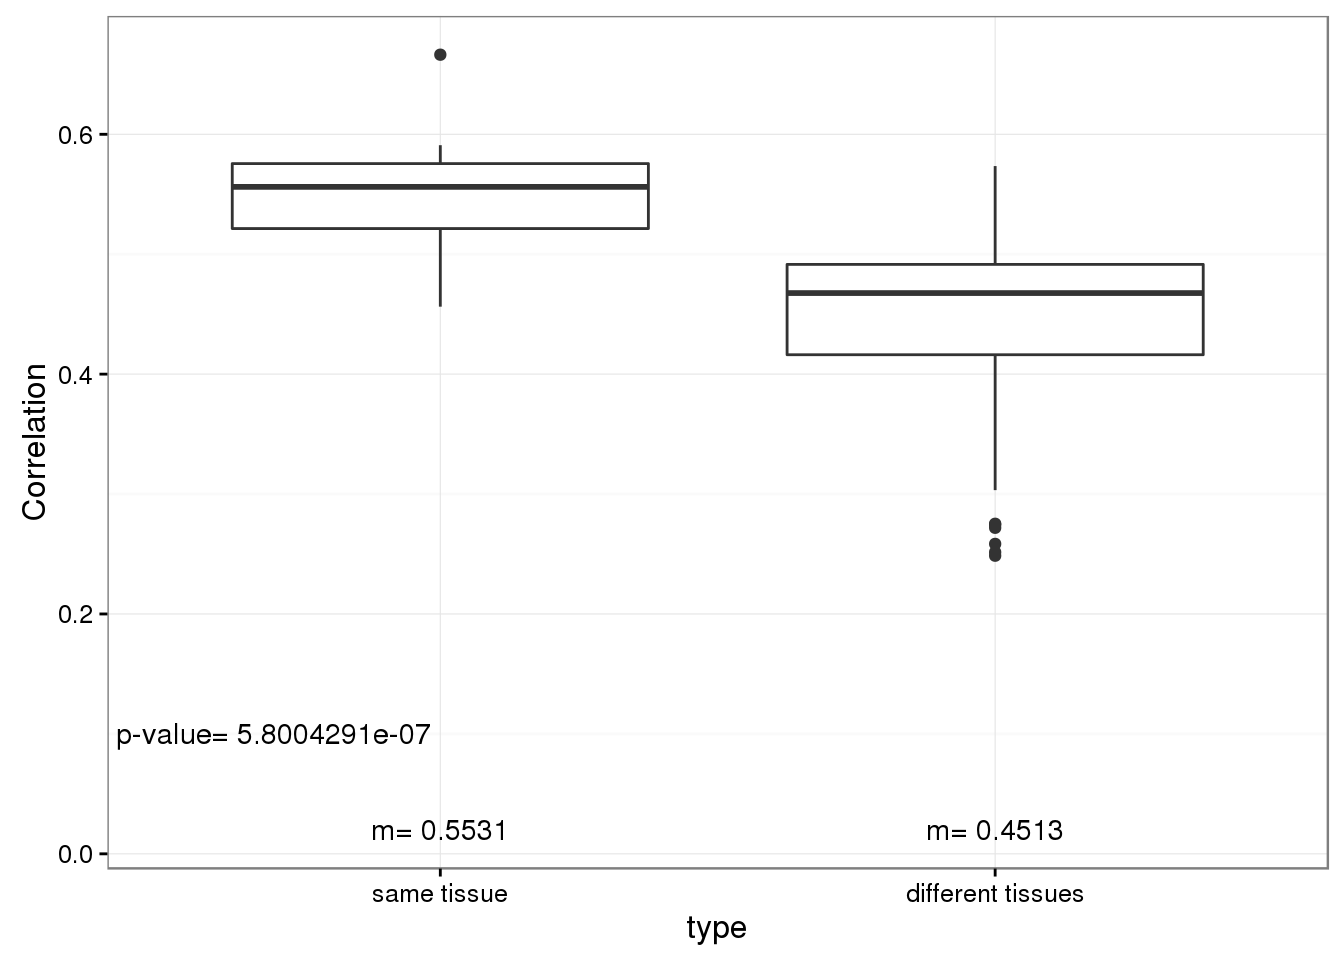
\includegraphics[scale=0.55]{integration/TestWhole_withoutLow.png}\centering
    \caption[Distribution of Pearson correlation coefficients for same tissue
    pairs versus random tissue pairs]{\label{fig:TestSig}\textbf{Distribution of
    Pearson correlation coefficients for same tissue pairs versus random tissue
    pairs.} The left boxplot displays the distribution of Pearson correlation
    coefficients for same tissues pairs (\eg\
Proteome\textsubscript{\tissue{Liver} }$\sim$Transcriptome\textsubscript{\tissue{Liver} }
or
Proteome\textsubscript{\tissue{Heart} }$\sim$Transcriptome\textsubscript{\tissue{Heart} }).
    \\The right boxplot shows the correlation of all the possible random
    pair of tissues (\eg\
Proteome\textsubscript{\tissue{Lung} }$\sim$Transcriptome\textsubscript{\tissue{Liver} }
or
Proteome\textsubscript{\tissue{Heart} }$\sim$Transcriptome\textsubscript{\tissue{Kidney} }).
    A Welch t-test has been performed to test the significance of the
    difference of the means of the two groups ($0.55$ for the same tissue and
    $0.46$ for the random pairs). The difference is significant under the null
    hypothesis $H_{0}$ (The mean of the same pair-tissue coefficient correlations
    is higher than the random tissue pairs for a confidence interval of $95\%$:
    p-value: $5.8e-07$).}
\end{figure}

\TK{citation for Welch t-test}

\TK{transition: we know that the overall expression profiles are closely associated.
Next point is to check if a higher specificity of the proteome of a tissue is due
to a greater specificity at transcriptome level.}

\subsection{Uniqueness of a protein can not be deduced by the uniqueness of a
\mRNA}
If we consider \cref{fig:KusterPandeyFQM},
(particularly \cref{fig:KusterPandeyFQM}|C), we can see that for every tissue,
there are proteins only detected in that specific tissue. This is also the case
for the transcriptome, some \mRNAs\ have been detected in only one tissue.
\Cref{fig:barPlotunique0nb} shows the amount of \mRNAs\ and proteins that have
been \emph{detected} in each tissue. The number of \mRNAs\ is actually quite
high. However, the limit of detection for \mRNAs\ does not imply that these \mRNAs\
are translated into proteins or that they are specific to the tissue. Indeed,
as I have presented previously (see~\Cref{ch:Transcriptomics}),
most of the \mRNAs\ are detected everywhere.

Hence, as a second approach, I only used the \mRNAs\ expressed
above $1$ \gls{FPKM} (see \cref{fig:barPlotunique1nb}). Independently of
thresholds, \tissue{Testis} presents --- consistently --- the highest number
of unique proteins and \mRNAs. We can also observe that the number of \mRNAs\
detected is roughly equivalent to the number of \mRNAs\ quantified only once at
least at (or greater than) $1$ \gls{FPKM} although these \emph{unique} genes are
not exactly the same.

As there is an obvious bias towards the low expressed \mRNAs\
(which are usually part of the least correlated pairs of \mRNA/proteins), I also
used a threshold of 5 \glspl{FPKM}. This last threshold, albeit purely arbitrary,
has already been used in the literature and presents some similarity regarding the
breadth of expression of \mRNAs\ with the proteins' one
(see \cref{subsec:IntegrationProteinBimodalExpre}).

\TK{insert reference here --- check cancer studies}

At this threshold, the number of \emph{unique} \mRNAs\ is lesser than previously,
but still greater than the number of \emph{unique} proteins (see
\cref{fig:barPlotunique5nb}).

Once again, there is a lack of any obvious relation between
the proteomic and transcriptomic observations.
In \cref{fig:barPlotunique5ratio}, I used the ratio of the number of \emph{unique}
\mRNAs\ per tissue divided by the total amount across all the tissues.
Hence, we can easily see that while \tissue{Testis} presents more than half of
the \emph{unique} \mRNAs\, it represents less than a quarter of the diversity
at proteomic level.

\begin{figure}[!htbp]
    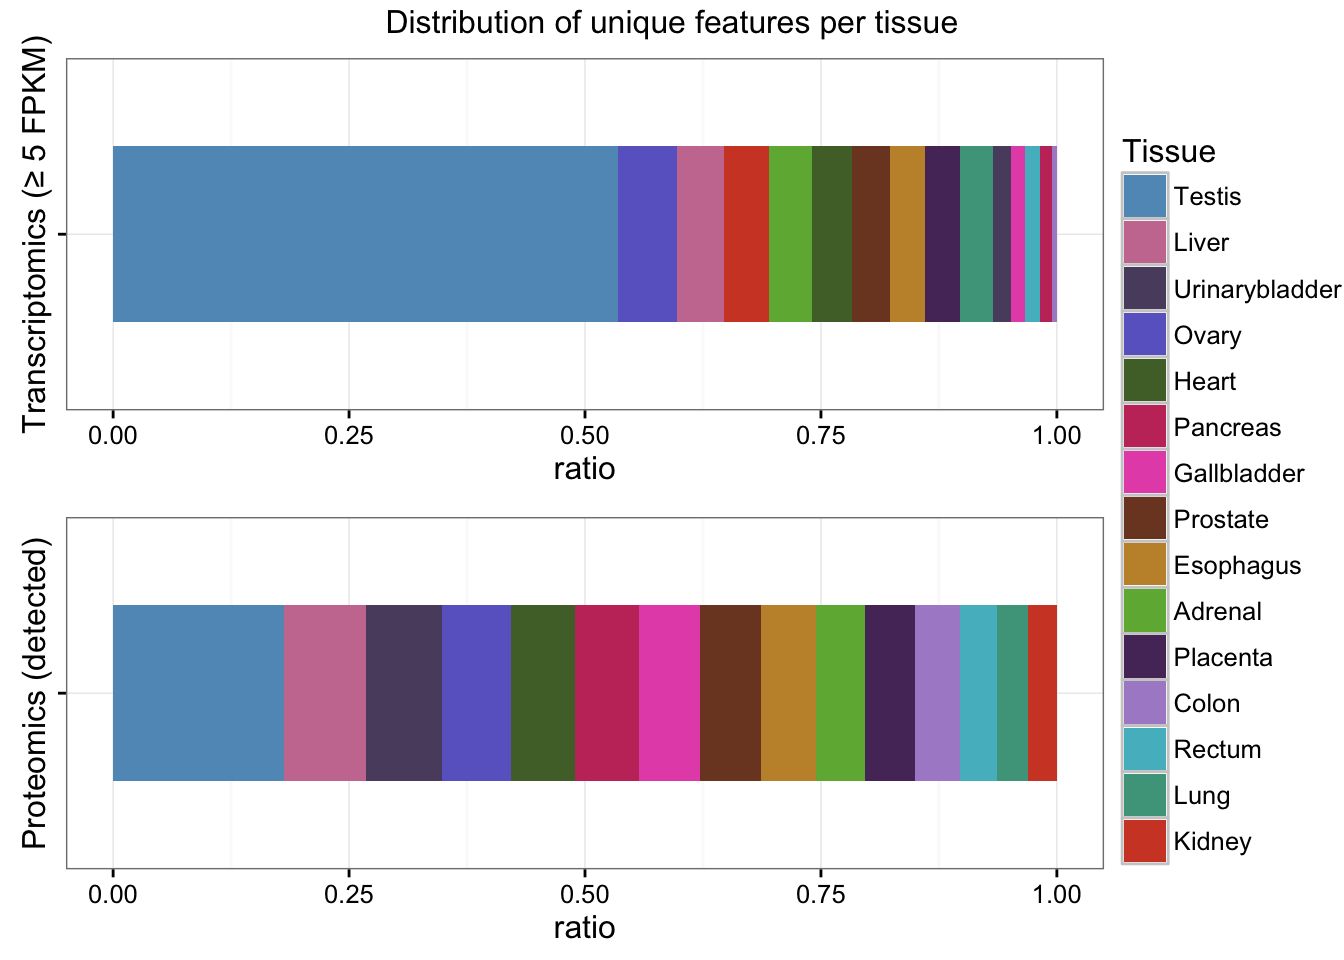
\includegraphics[scale=0.30]{integration/barPlotunique5ratio}\centering
     \caption[Distribution of \mRNAs\ and proteins detected (at specific
     thresholds) only in one unique
     tissue]{\label{fig:barPlotunique5ratio}\textbf{Number of
     \mRNAs\ (top) and proteins (bottom)
     that have been detected and quantified (\geq\ 5 \glspl{FPKM} for \mRNA\;
     \textgreater\ 0 for proteins).} While some tissue can have
     consistently a higher
     specificity at proteomic and transcriptomic level, it is not true for all.}
\end{figure}


\subsection{Distribution of expression breadth of the proteome is bimodal. As is
the expression breadth of the mRNAs --- if we apply a threshold}
\label{subsec:IntegrationProteinBimodalExpre}
\TK{this probably need to go to the previous chapters!}

In our study, most proteins are detected in a very limited number of tissues (one
or two) or in all the tissues as it can be observed in~\cref{fig:breadthProt}.
Overall, we found that most proteins are found in one tissue. We refer to them as
\emph{tissue-specific}.

\begin{figure}[!htbp]
    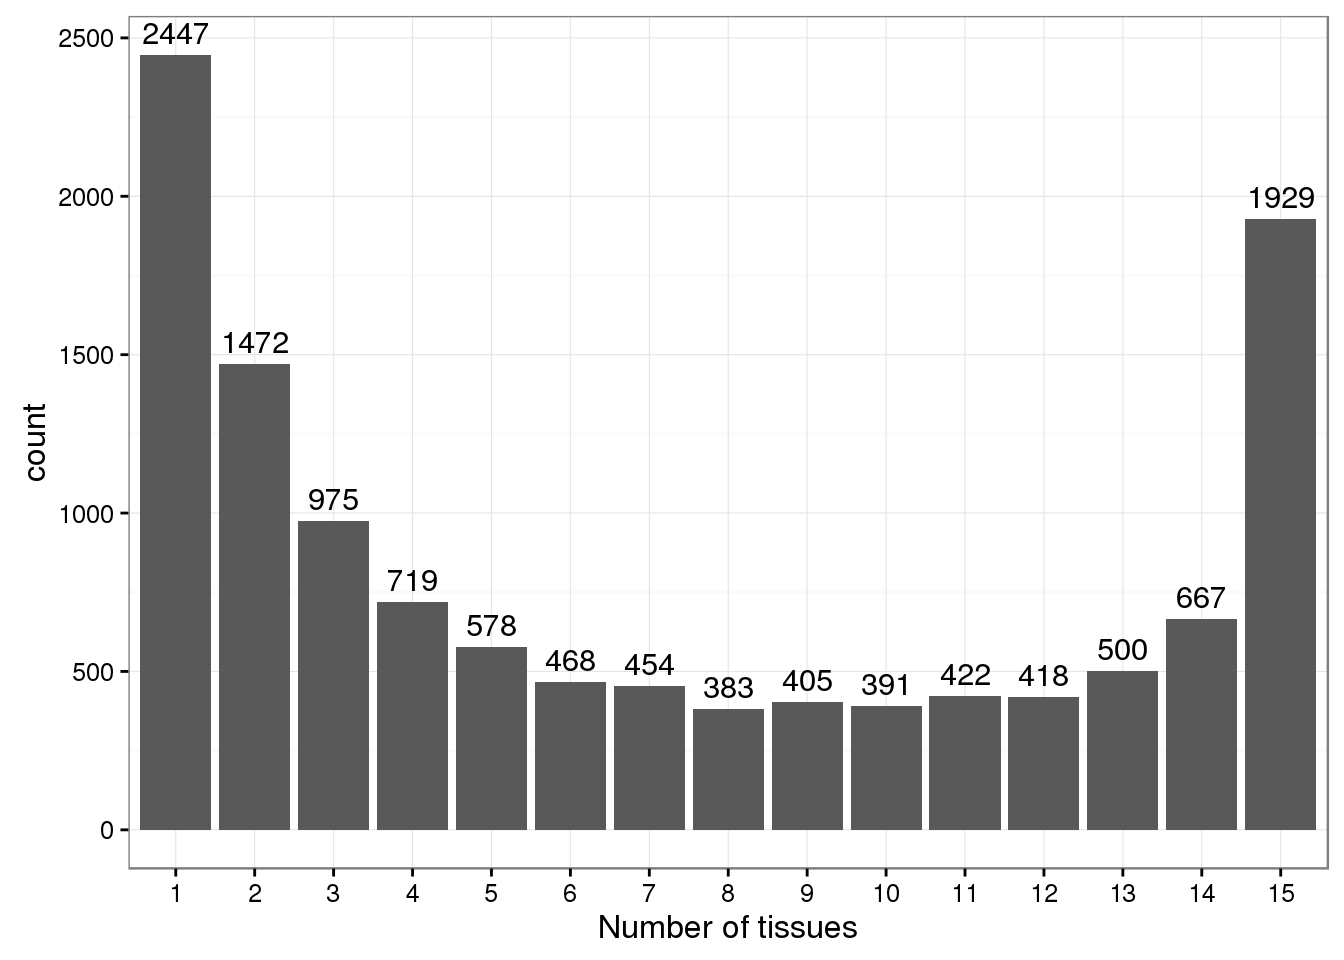
\includegraphics[scale=0.65]{integration/breadthProt.png}\centering
    \caption[Distribution of expression breadth for the proteome]
    {\label{fig:breadthProt}\textbf{Distribution of expression breadth for the
    proteome.} The breadth of expression is bimodal: most of the proteins are
    only found in one tissue. The second largest group is consisting of
    the ubiquitous proteins. The third largest group is the group of the proteins
    that are expressed in two tissues.}
\end{figure}


For the transcriptome, if we focus only on the detected genes, we don’t observe
the same trend as showed in~\cref{fig:breadthTrans}|A.
However, when we apply a threshold, either $1$ \gls{FPKM}
(\cref{fig:breadthTrans}|C) or
5 \glspl{FPKM} (\cref{fig:breadthTrans}|D), to which the \mRNA\ expressions
have to be greater or at least equal, then the expression breadth distribution
of the \mRNAs\ is also bimodal.

\begin{figure}[!htbp]
    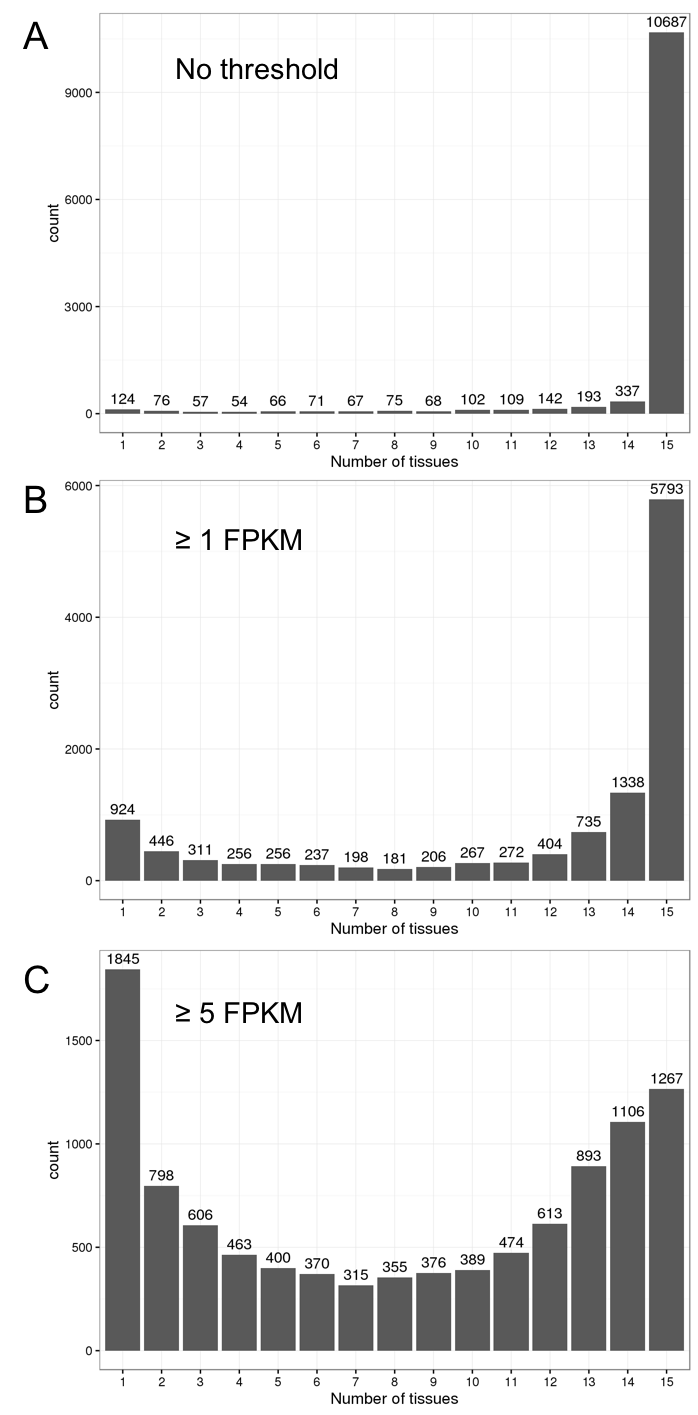
\includegraphics[scale=0.85]{integration/breadthTrans}\centering
    \caption[Distribution of expression breadth for the transcriptome]
    {\label{fig:breadthTrans}\textbf{Distribution of expression breadth for the
    transcriptome.} The distribution is given for several threshold.
    \textbf{A}| Every time a \mRNA\ is detected ($> 0$ \gls{FPKM}).
    \textbf{B}| Every time a \mRNA\ is detected at or above $1$ \gls{FPKM} and
    \textbf{C}| $5$ \glspl{FPKM}.}
\end{figure}

\subsection{Few protein expression breadth can be predict by transcript
expression breadth}

\begin{figure}[!htbp]
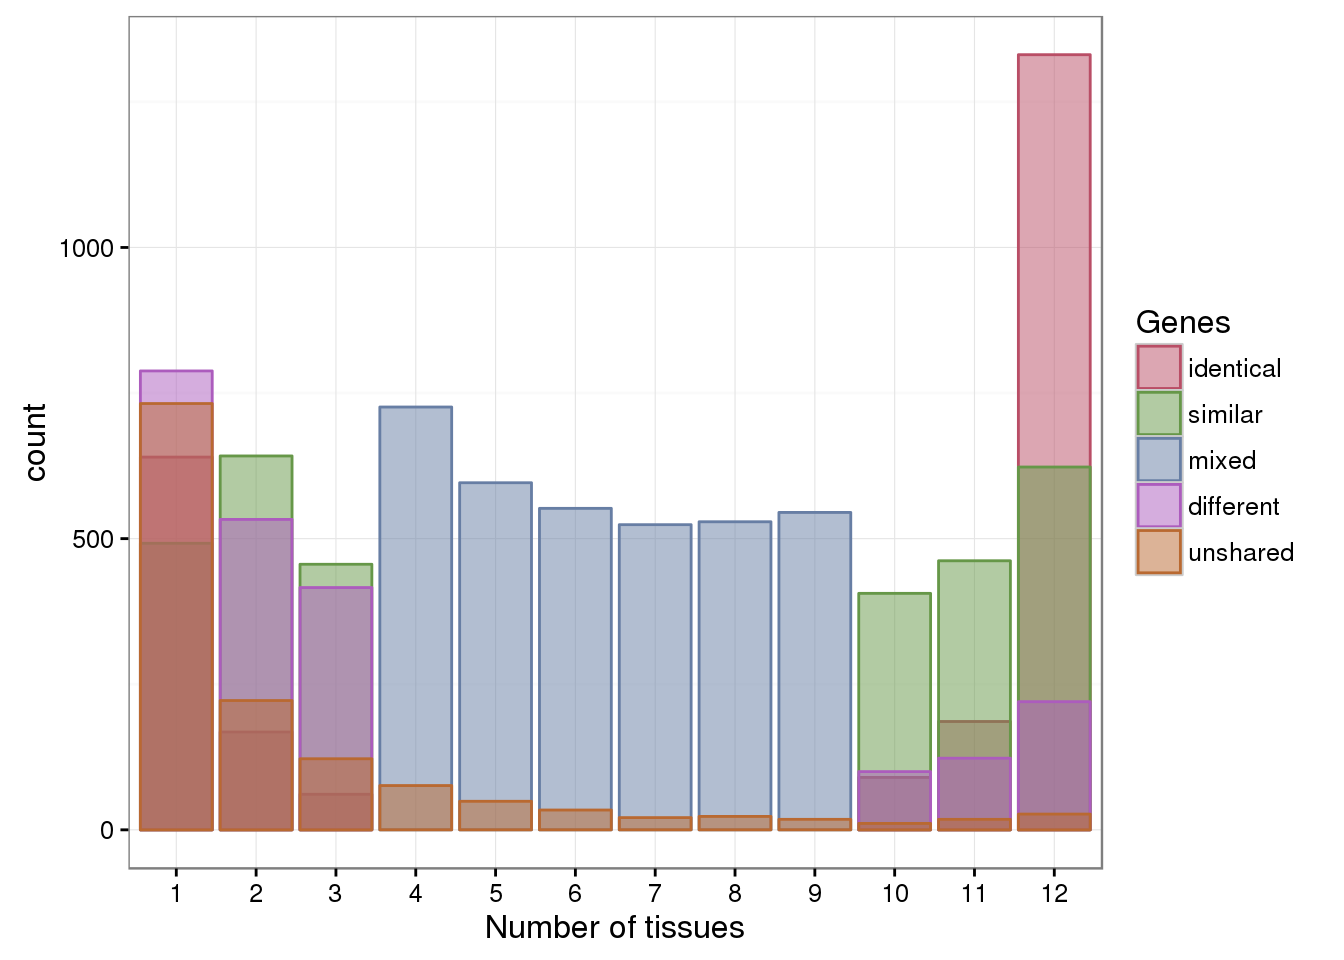
\includegraphics[scale=0.30]{integration/PandeyUhlenAnnoBreadth}\centering
    \caption[Proteome expression breadth compared to the transcriptomic one]{\label{fig:breadthColPandeyUhlen}\textbf{Proteome expression breadth
    compared to the transcriptomic one.}The breadth of expression of each protein
    is compared to the breadth of its corresponding \mRNA\. Several possible cases
    are showed. Some proteins haven't been found in the transcriptomic samples,
    they are \emph{unshared.}
    The breadth can be \emph{identical}:the protein and the \mRNA\ are
    expressed in the same number of tissues. The first and last three columns
    have been grouped together. If a protein and its \mRNA\ are in the same group,
    they are tagged as \emph{similar}. If the protein and the \mRNA\ are both
    expressed between 4 to 9 tissues, they are described as \emph{mixed}. If the
    pair is not belonging to any of the previous categories, it is then described
    as \emph{different}.}
\end{figure}

\TK{While the unique protein/\mRNA\ are not concluant; the next analysis was to
determine if the closeness of two tissues are conserved between proteomic and
transcriptomic tissues.}

\subsection{Tissue clusters differ between Proteomic and Transcriptomic}
\begin{figure}[!htbp]
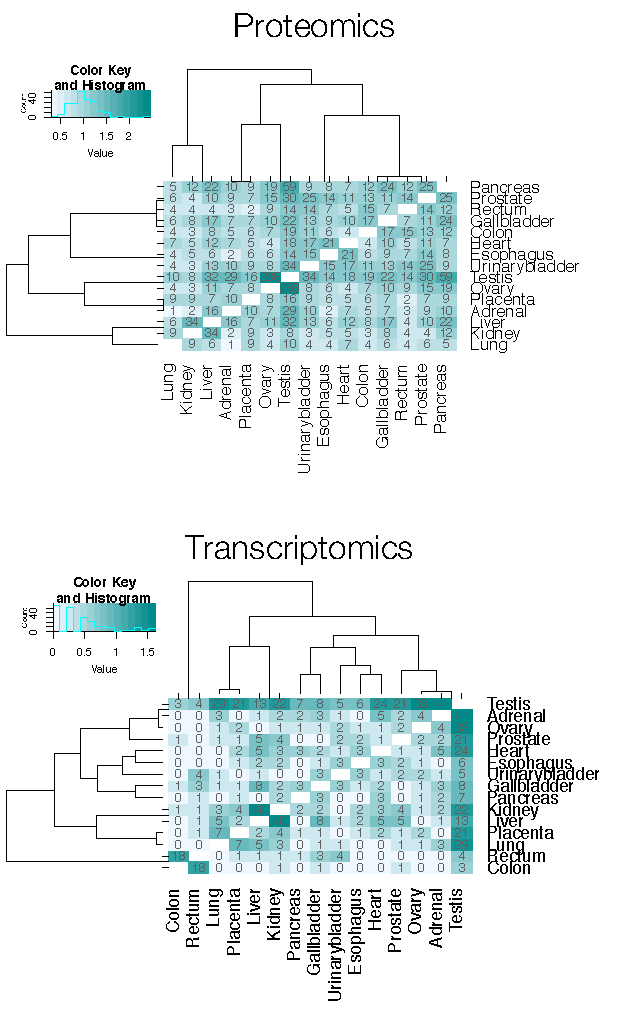
\includegraphics[scale=0.8]{integration/heatmapPairs}\centering
    \caption[Clusters of tissues based on number of proteins or \mRNAs\ shared
    between a pair of tissues]{\label{fig:heatmapPairs}\textbf{Clusters of
    tissues based on number of proteins or \mRNAs\ shared between a pair of
    tissues.} For each pair of tissues, I have collected the number of proteins
    (or \mRNAs) expressed only in that pair. That number is displayed in the
    cell. The heatmap is a symmetric heatmap. Higher is the number of features
    (proteins or \mRNAs) shared between two tissues and closer they are
    considered. We can observe that the tissue presenting the most shared features
    with the other tissues is \tissue{Testis}.}
\end{figure}

\TK{Comparison of the two trees}

\begin{figure}[!htbp]
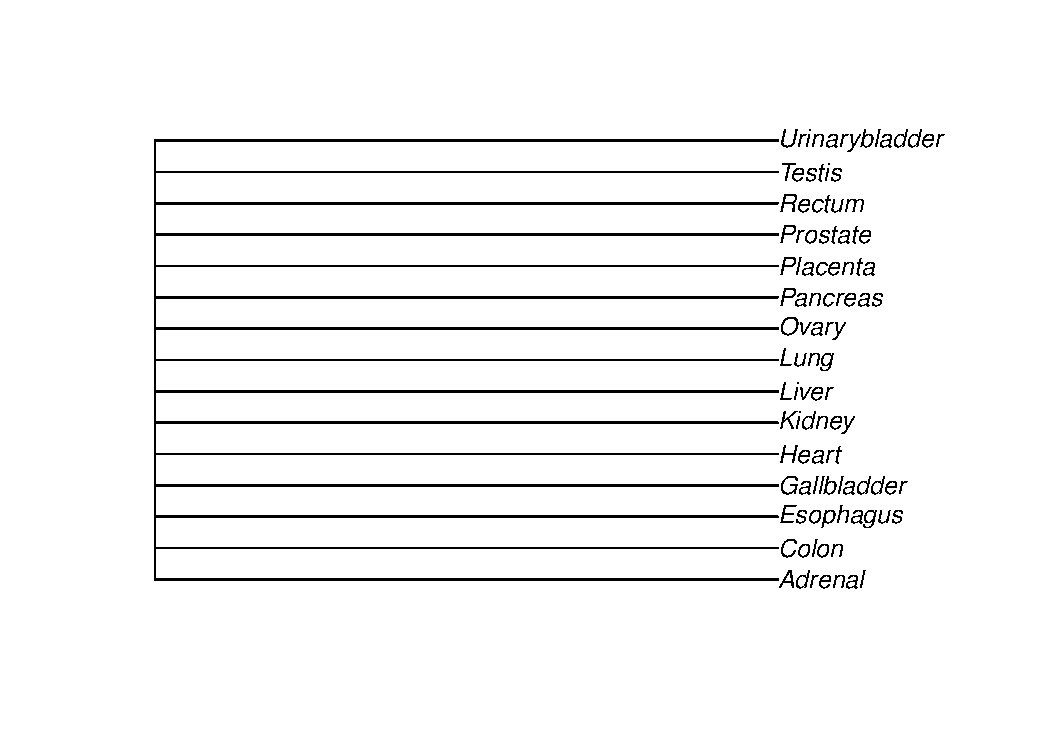
\includegraphics[scale=0.7]{integration/consensusTree}\centering
    \caption[Consensus tree between the cluster trees of the proteome and the
    transcriptome]{\label{fig:consensusTree}\textbf{Consensus tree between the
    cluster trees of the proteome and the transcriptome.}}
\end{figure}

It appears that a direct comparison of the proteins that have been identified
with the identified \mRNAs\ (even with various thresholds) is not so meaningful.

Instead of focusing of the uniqueness of a gene (or in a broader way, the breadth
of expression),the main issue here is to
determine what and when a gene is \emph{specific}. In fact, I can not use
the same definition of detection like for the proteins. I then chose to focus
on the \emph{Tissue-Specific} genes.

\subsection{Tissue specific \textit{m}RNAs have significant overlap with tissue
specific proteins}

\begin{figure}[!htbp]
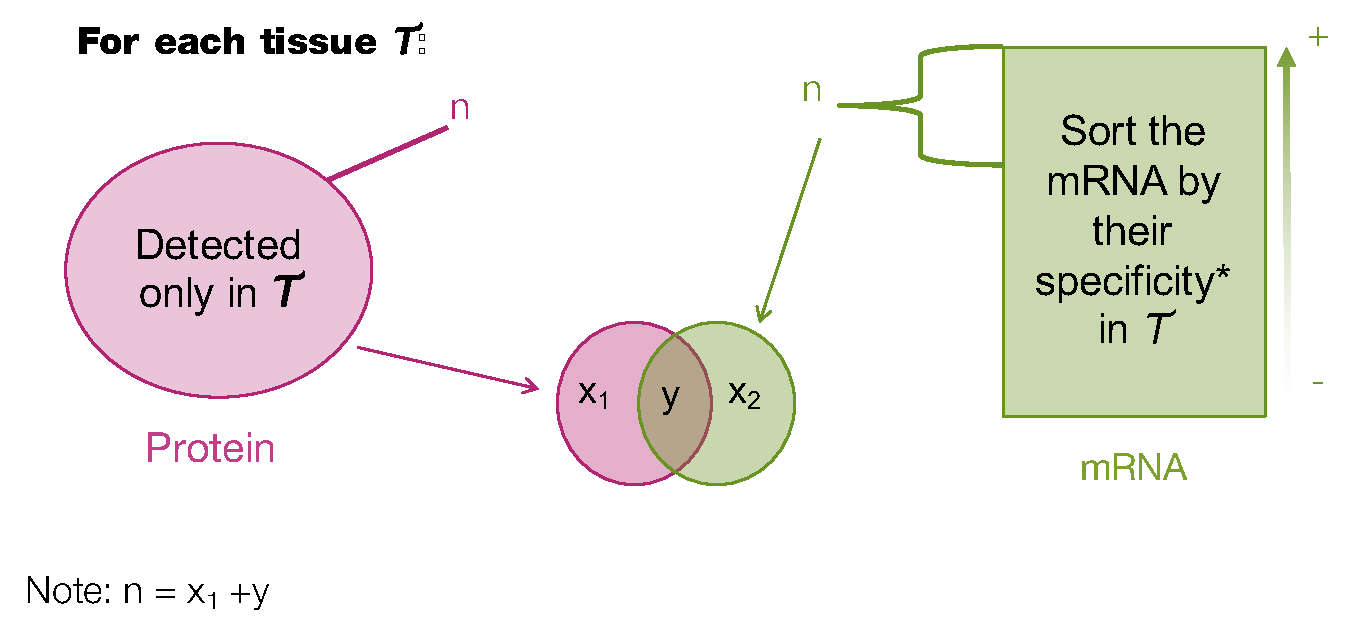
\includegraphics[scale=0.7]{integration/RankSpe}\centering
    \caption[Determination process of specific
    mRNAs]{\label{fig:RankSpe}\textbf{Determination process of specific \mRNAs.}}
\end{figure}


\begin{figure}[!htbp]
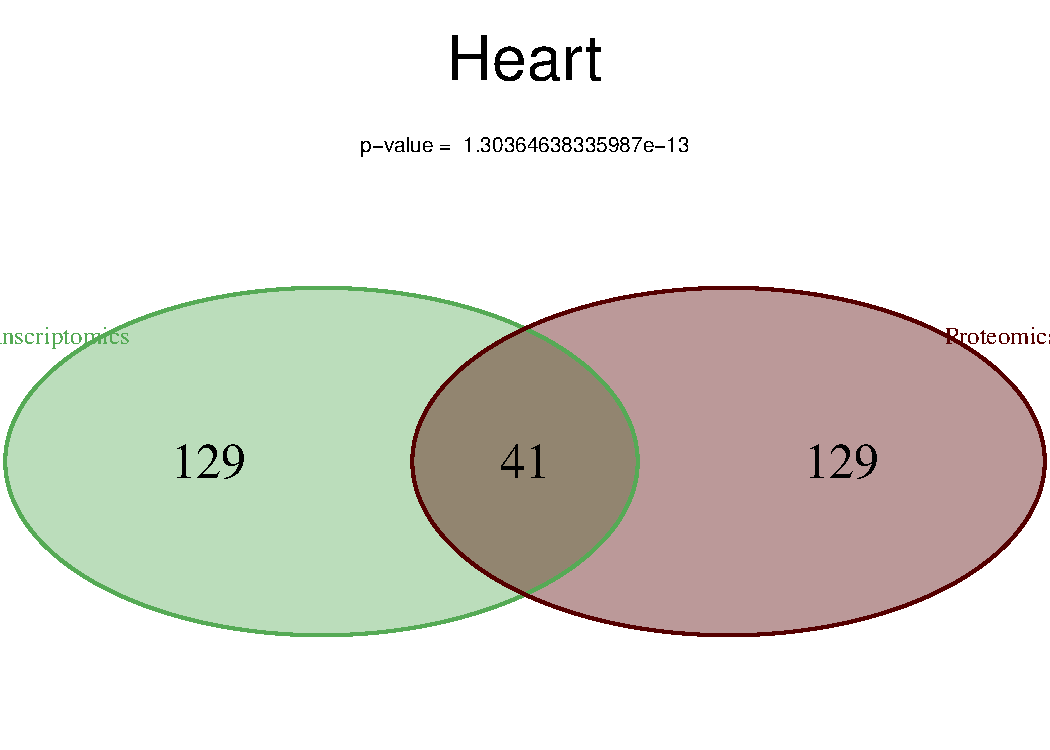
\includegraphics[scale=0.7]{integration/SpeJacquard/Heart}\centering
    \caption[Example of overlap of specific protein and specific
    mRNAs for heart]{\label{fig:ExJacquard}\textbf{Example of overlap of
    specific proteins and specific \mRNAs.}}
\end{figure}


\begin{figure}[!htbp]
\includegraphics[scale=0.4]{integration/RatioJac}\centering
    \caption[Heatmap of Jaquard indices]{\label{fig:RatioJac}\textbf{Heatmap of
    Jaquard indices.}}
\end{figure}

\begin{figure}[!htbp]
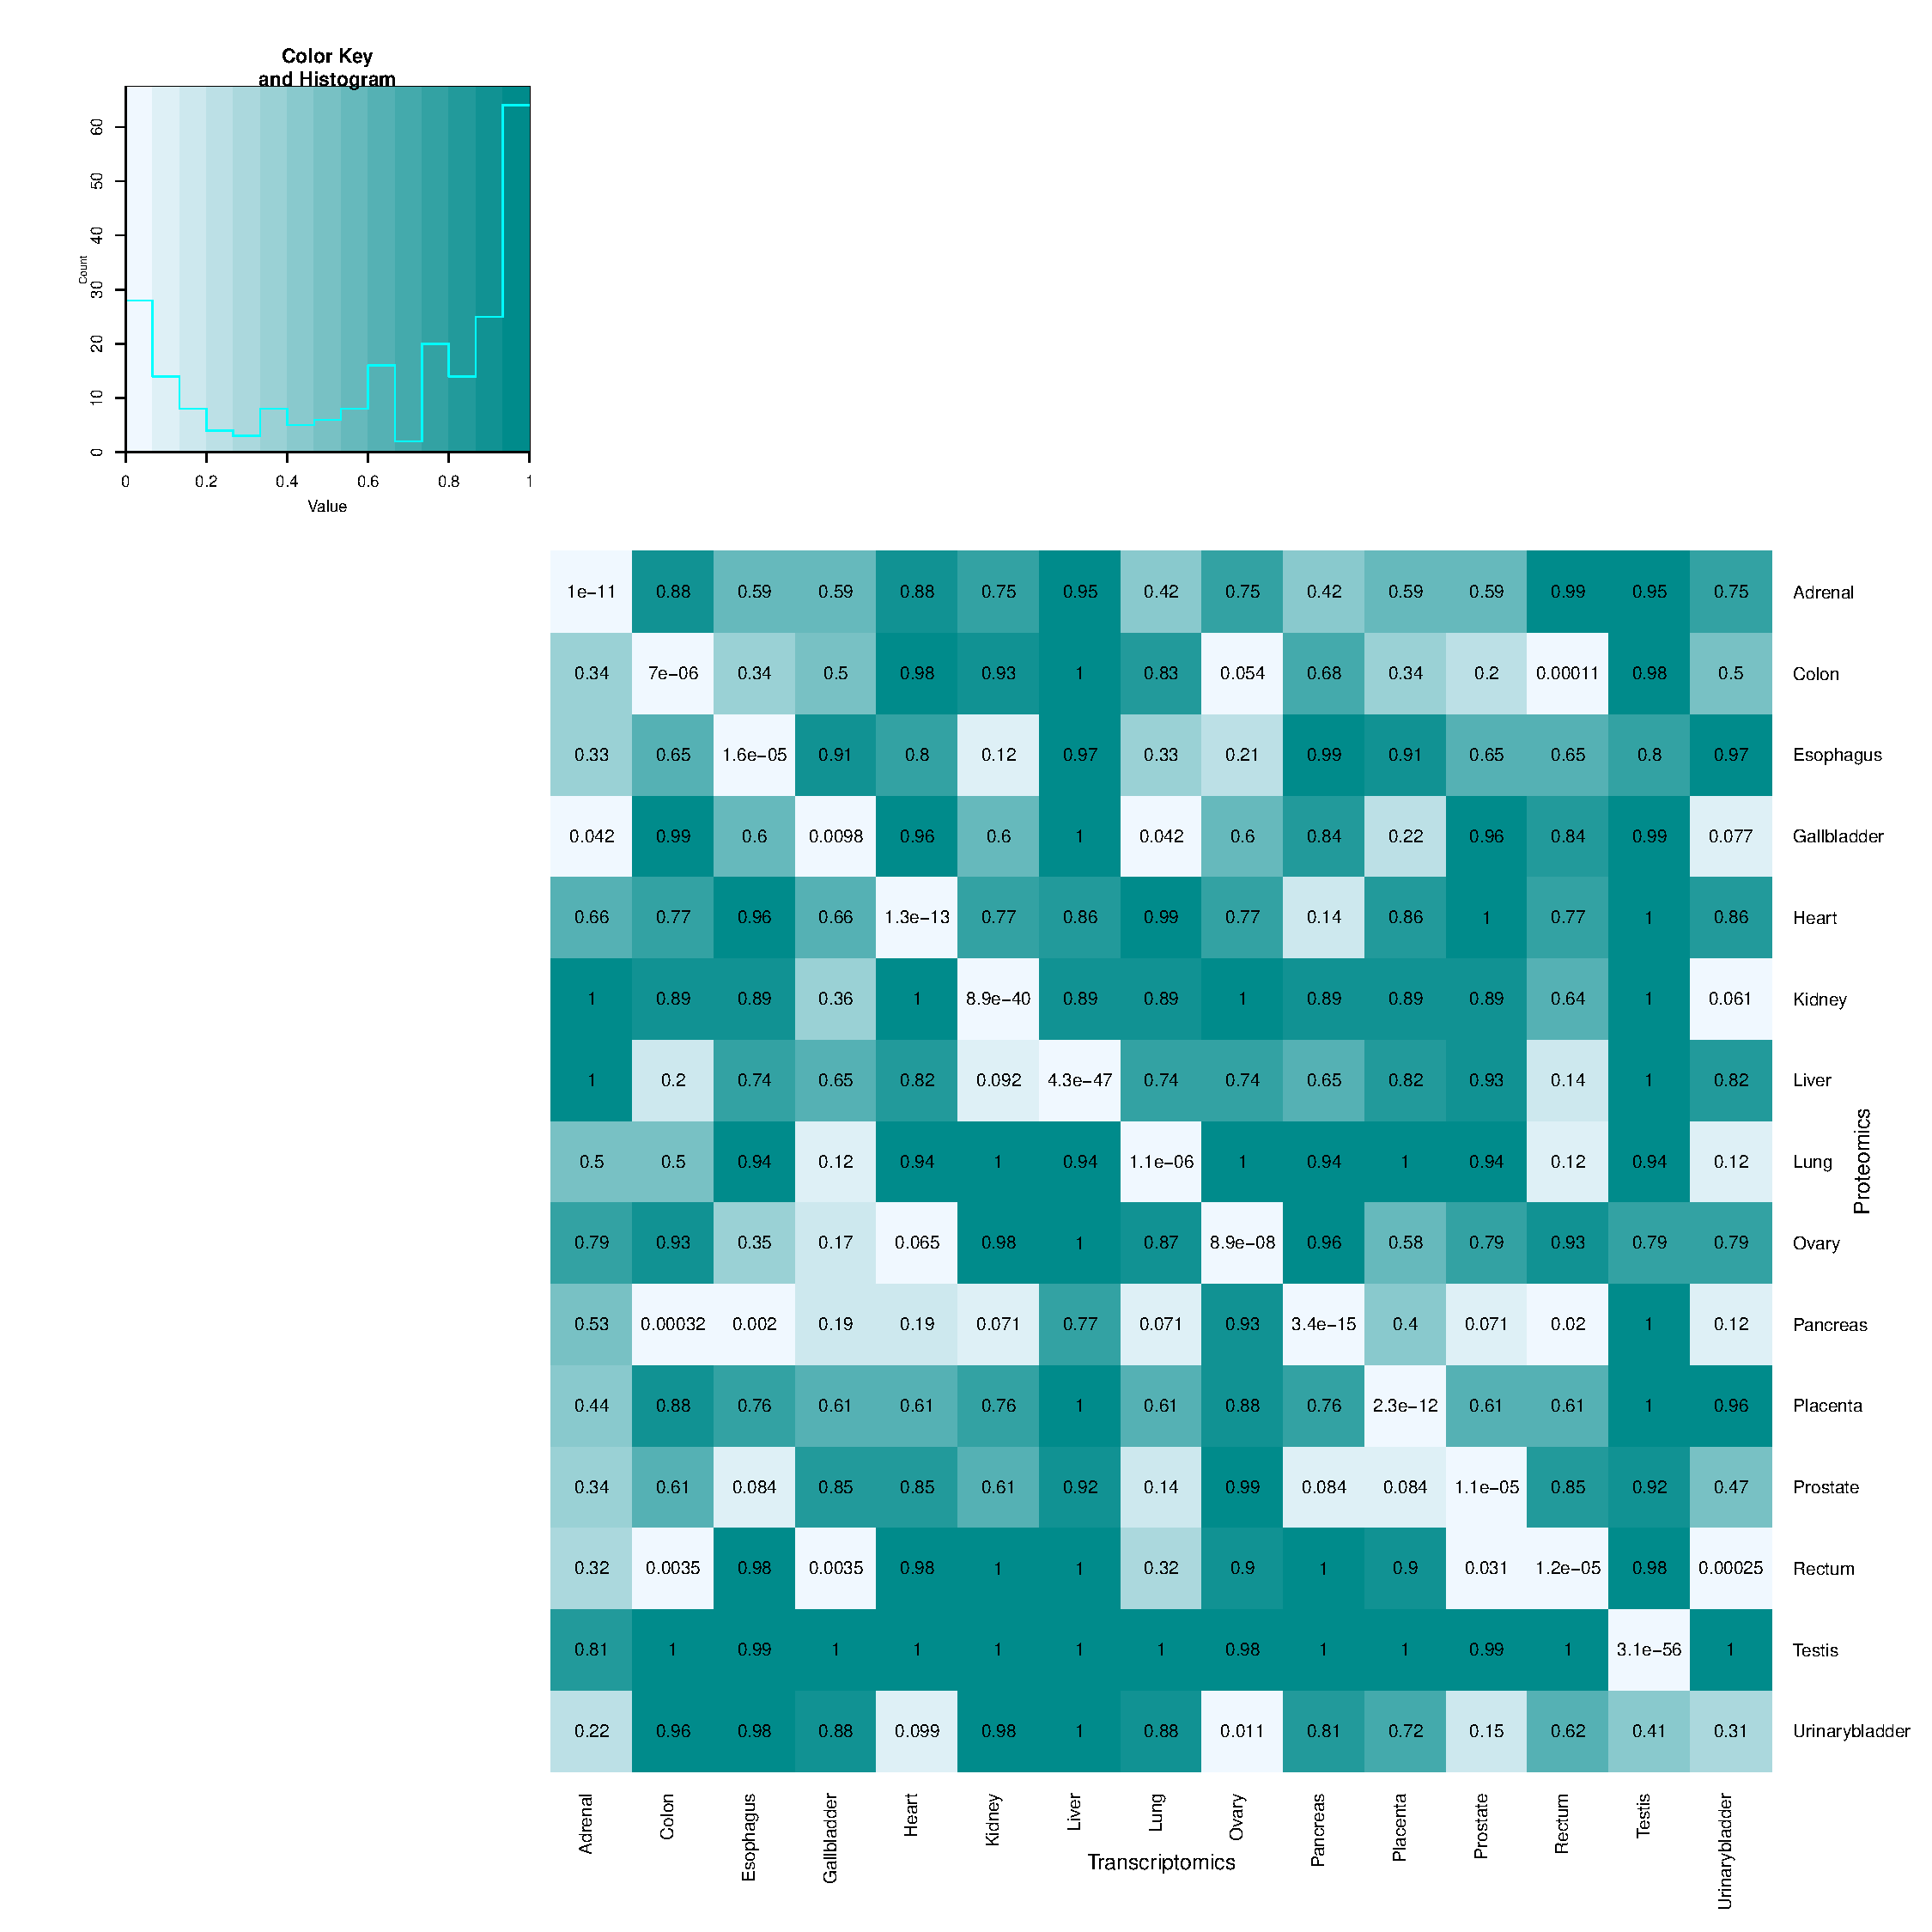
\includegraphics[scale=0.4]{integration/pJacquard}\centering
    \caption[p-values associated to the Jaquard
    indices]{\label{fig:pJacquard}\textbf{p-value associated to the Jaquard
    indices.}They have been computed with hypergeometric test.}
\end{figure}

\subsection{Expression levels of mRNAs correlate with the expressed proteins}

\begin{figure}[!htbp]
    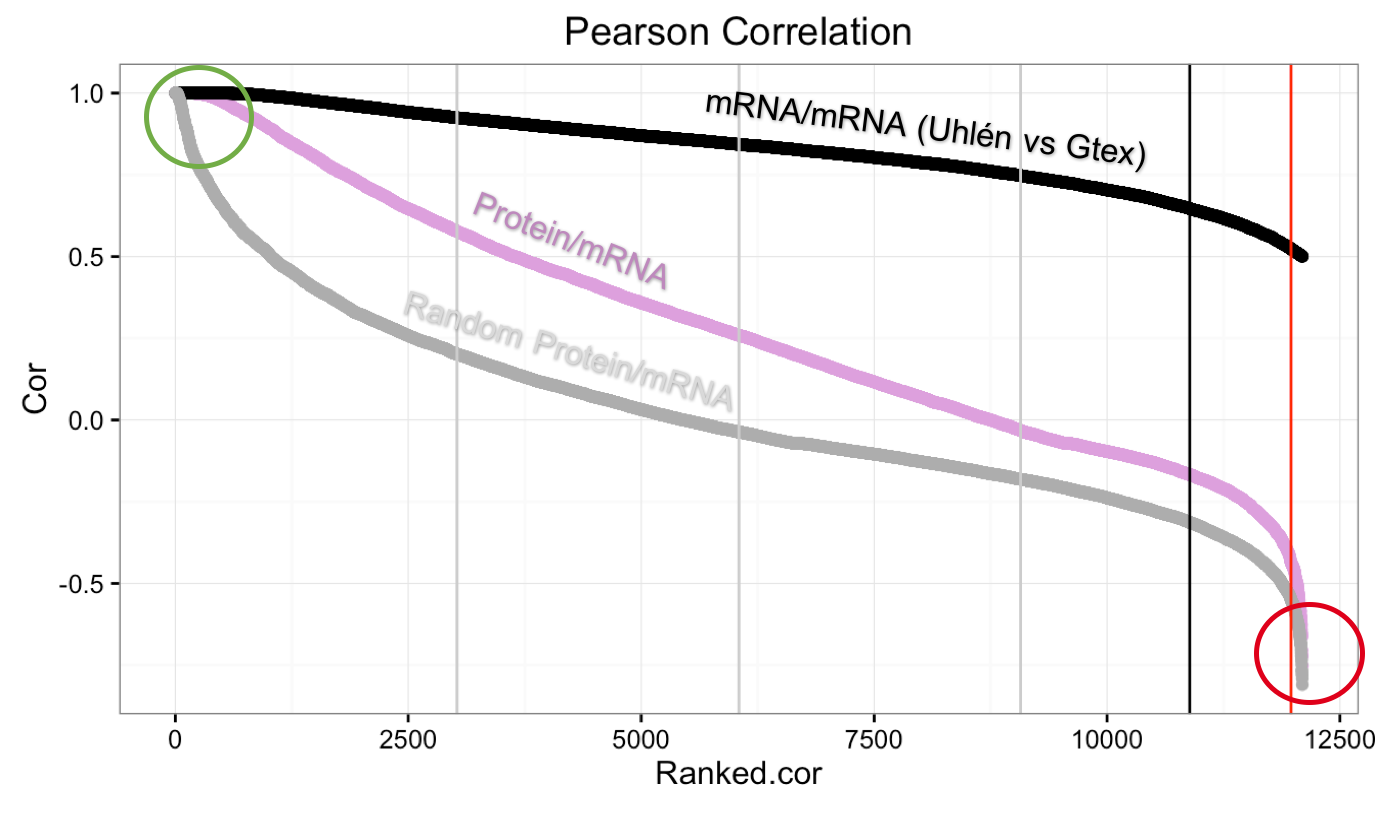
\includegraphics[scale=0.55]{integration/GeneProtCorAnno}\centering
    \caption[Pearson correlation coefficients of \mRNA/protein pairs expression
    across the common tissues in descending order]
    {\label{GeneProtCor}\textbf{Pearson correlation coefficients of \mRNA/protein
    pairs expression across the common tissues in descending order.} For each
    couple of \mRNA\ and its corresponding protein, the Pearson correlation of
    their respective expression across the same set of tissue is calculated. Then,
    all the pairs are sorted in descending order and plotted based on their
    correlation coefficient in pink. To provide context to these results,
    An \emph{ideal} case has also been calculated. The identical \mRNAs\ set of
    the current Proteome and Transcriptome comparison has been used for a
    Transcriptome (\dataset{Uhlén \etal}) and Transcriptome comparison
    (\dataset{GTEX}). We can see that even the ideal case is not a perfect
    horizontal line (which would indicate a whole and complete correlation between
    the two transcriptomic datasets).}
\end{figure}


\begin{figure}[!htbp]
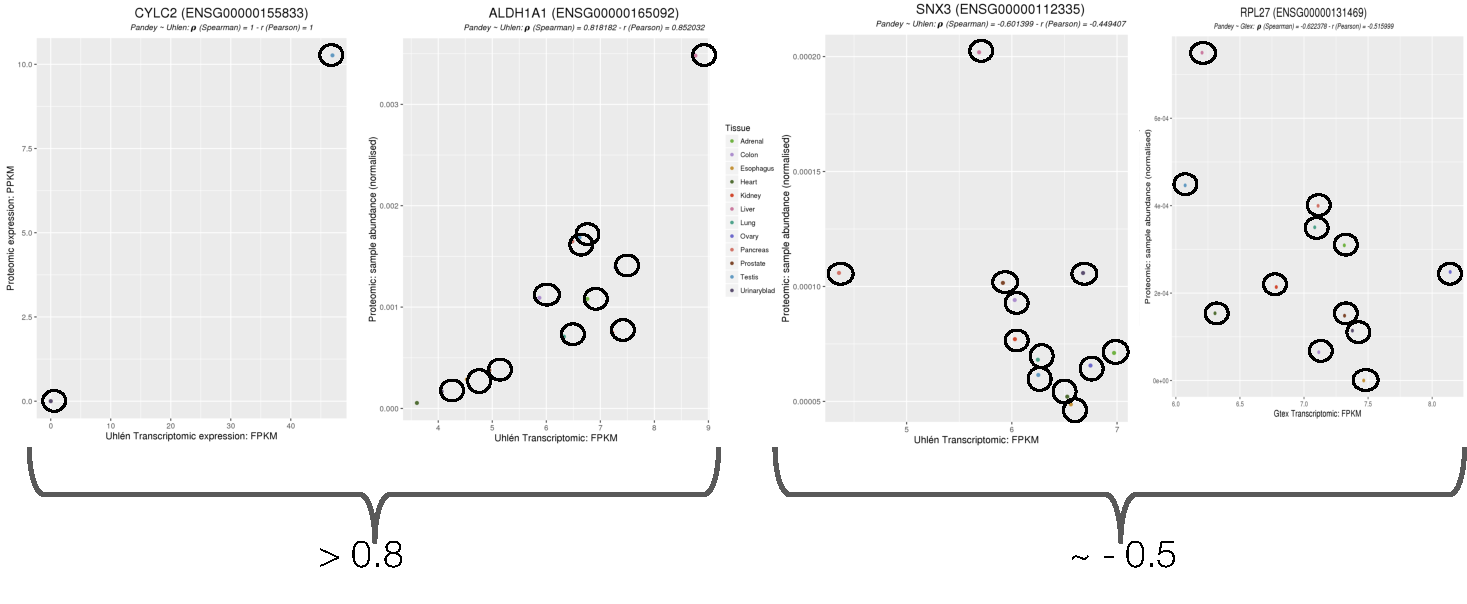
\includegraphics[scale=0.5]{integration/caseGene}\centering
    \caption[Different cases of correlation
    protein/mRNA]{\label{fig:caseGene}\textbf{Different cases of correlation
    protein/\mRNA.} The high correlated ones are enriched in pairs that are
    Tissue-specific as \mRNA\ and protein.}
\end{figure}

\subsection{Pairs composed of tissue specific proteins tend to correlate better}

\begin{figure}[!htbp]
    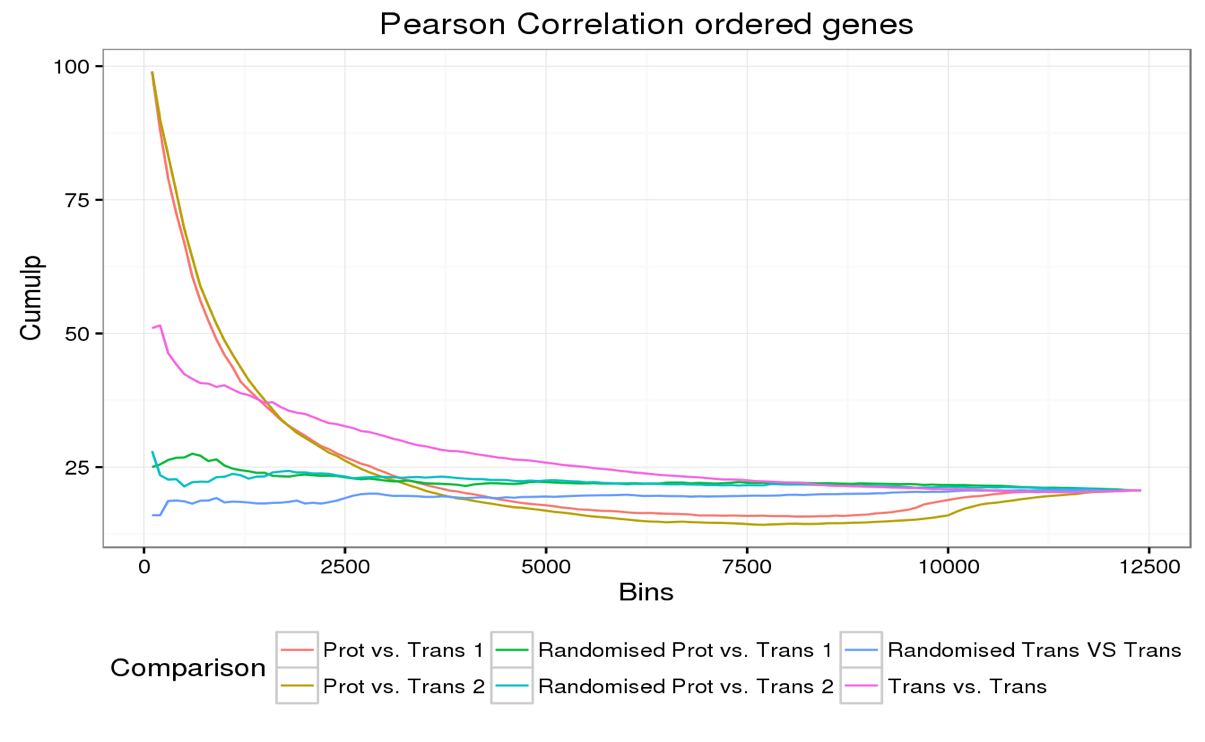
\includegraphics[scale=0.7]{integration/Spe_Cor}\centering
    \caption[Cumul ratio of the specific proteins ordered on the correlation
    of the mRNA/protein pairs across the 15
    tissues]{\label{fig:Spe_Cor}\textbf{Cumul ratio of the specific proteins
    ordered on the correlation of the mRNA/protein pairs across the 15 tissues.}}
\end{figure}


\TK{Can tissues correlations be improved by removing the lowly correlated genes? =>
it is not always the same pairs that are in the same quadrant ==> no `argument''
that would legitimate this. Ref:~\cref{fig:CorImprovable}}


\begin{figure}[!htbp]
    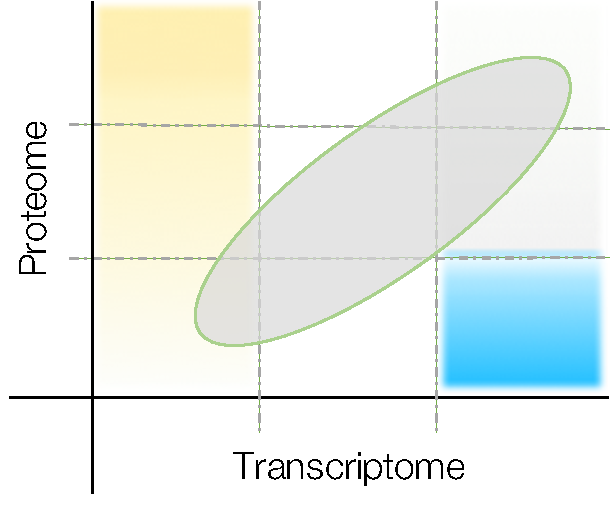
\includegraphics[scale=0.85]{integration/improvingTisseCor}\centering
    \caption[Possible biological significations of a \mRNA/protein pair based on
    its possition in the scatter plot]
    {\label{fig:CorImprovable}\textbf{Possible biological significations of a
    \mRNA/protein pair based on its position in the scatter plot.}Indeed, as all
    the scatter plots present the same shape with a saturation for the proteins
    highly expressed in each tissues and a great dispersion for the lowly
    expressed \mRNAs}
\end{figure}


\subsection{GO enrichment of the different categories}


\begin{figure}[!htbp]
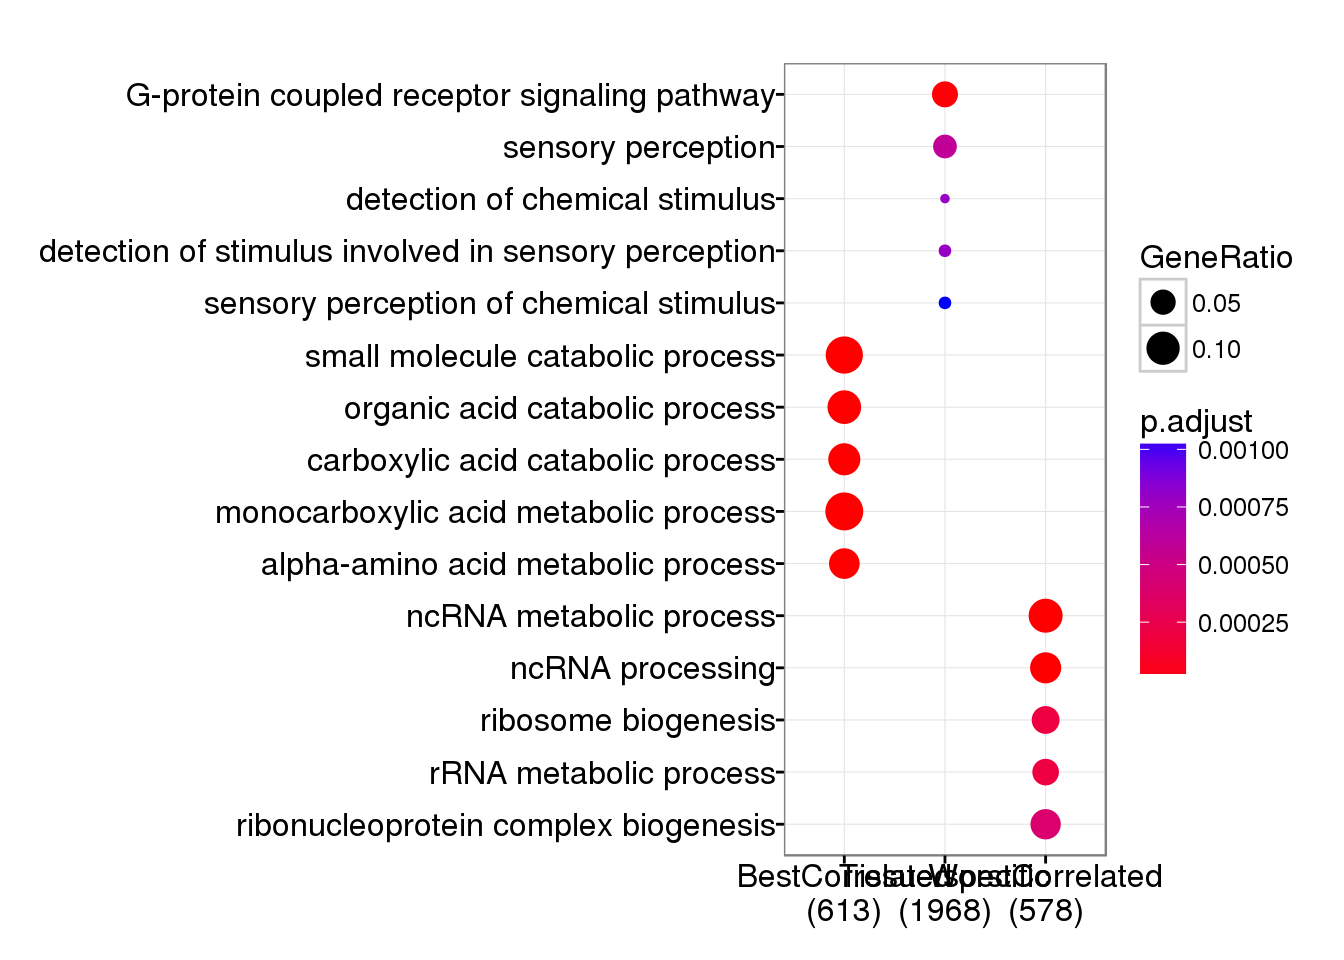
\includegraphics[scale=0.7]{integration/Go_dotplot}\centering
    \caption[GO enrichment analysis of the highest, lowest and Tissue
    specific genes]{\label{fig:Go_dotplot}\textbf{GO enrichment analysis of the
    highest, lowest and Tissue specific genes.}}
\end{figure}


\begin{figure}[!htbp]
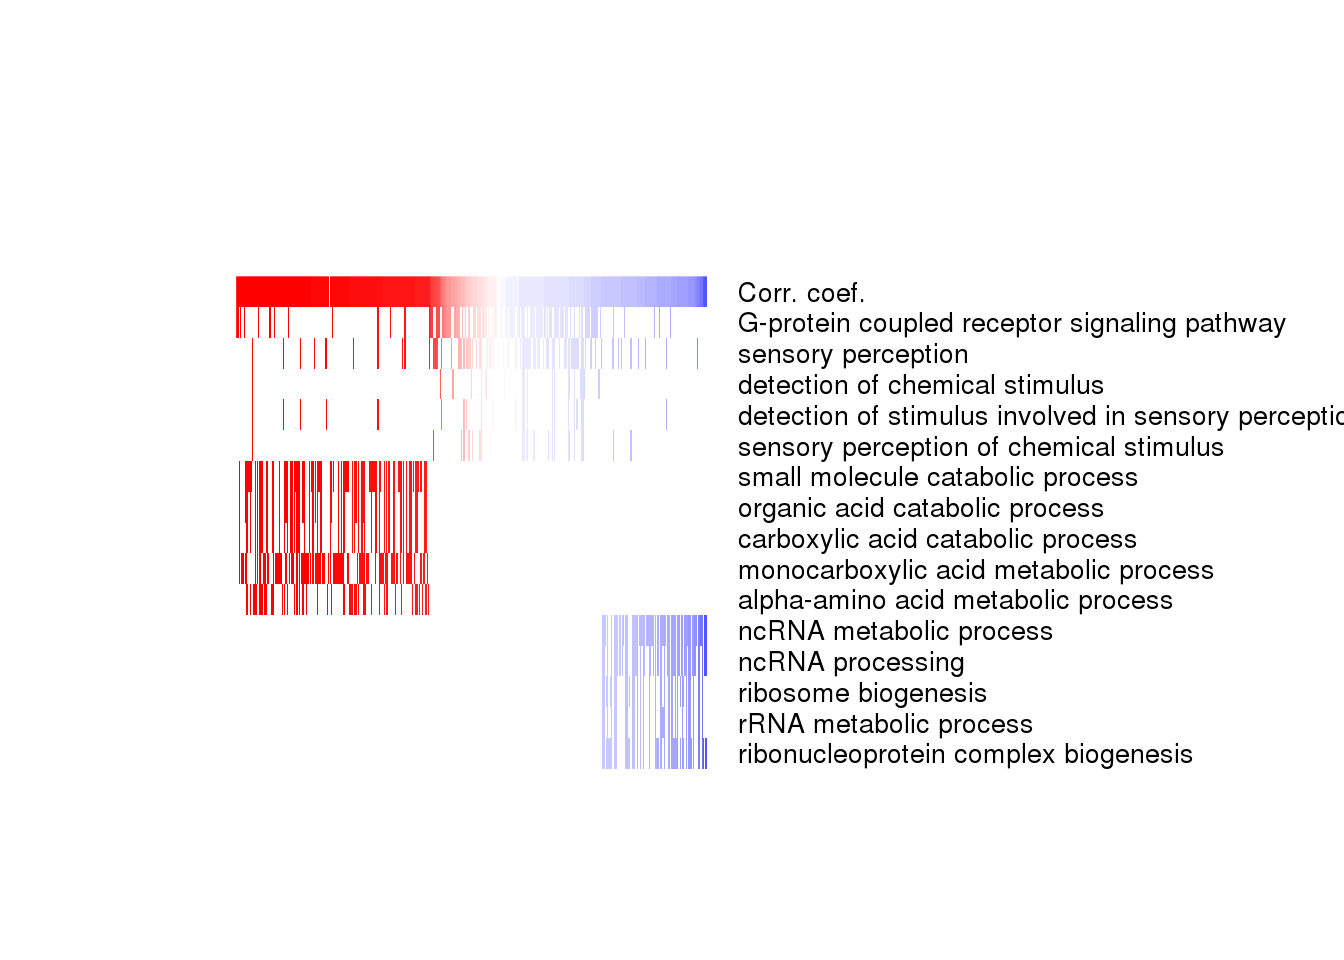
\includegraphics[scale=0.7]{integration/GO_cor_sorted}\centering
    \caption[Correlation coefficient of the pairs for the GO
    categories]{\label{fig:GO_cor_sorted}\textbf{Correlation coefficient of the
    GO categories.}}
\end{figure}


\begin{figure}[!htbp]
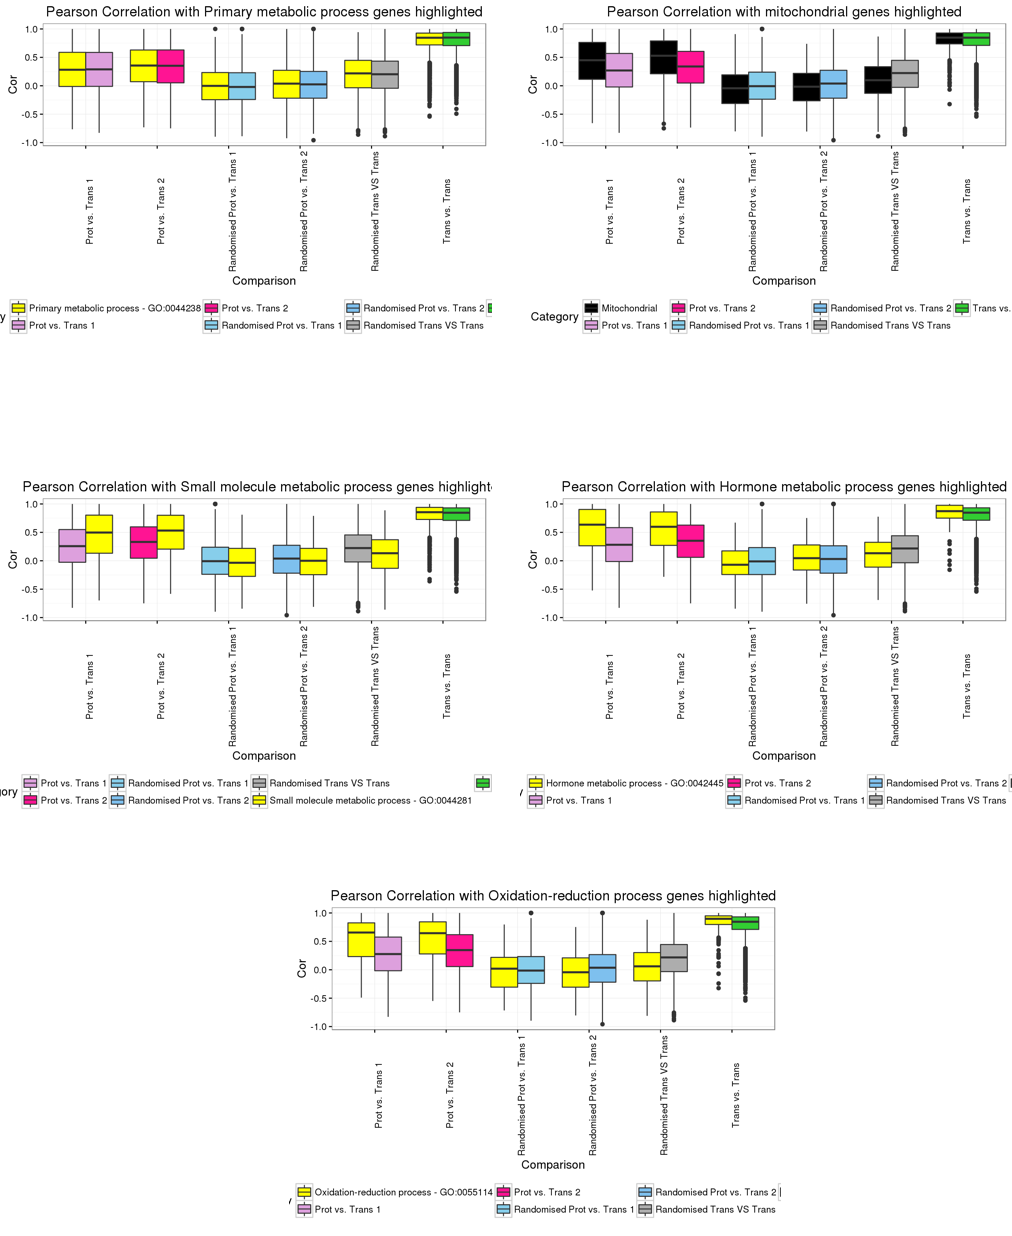
\includegraphics[scale=0.7]{integration/OtherGroups}\centering
    \caption[Examples of particular GO
    categories]{\label{fig:GO_sub_groups}\textbf{Examples of particular GO
    categories.}}
\end{figure}

%\begin{figure}
%    \includegraphics{integration/}\centering
%    \caption[]{\label{} \textbf{}
%    }
%\end{figure}

%if tissue more specific (greater diversity) the proteome, true for transcript as well?
%   barplot (no cutoff) but then 1FPKM<=> 1 protein (barplot 1FPKM ? yes/no?)
%        ---> breadth of expression distribution
%          ---> barplot 5 FPKM ==> Doesn't work BUT other way to compute the
%          specificity of mRNAs--> rank then compute Indice de Jacquard!
%===> *SO* specificity can be kept between Protein and Transcript
%_but then_ quid of Expression values, do they correlate?
%        * Eh, but then show that most high correlated are the specific but not only:
%        there are also others ---> GO annotation.



\clearpage\


\subsection{Annotation + Methodology impact}
\TK{comparison with the Scientific report paper}
And additionally the following idea.

At first, the quantification used for the proteomic data was following
state-of-the-art protocols for which we applied very stringent parameters:
to identify and quantify a given protein, three different unique peptides
(with an \gls{FDR} $< 0.01 \%$) have to be mapped solely to that protein.
A major issue of this approach is that many proteins have similar sequences;
hence, some peptides can only be attributed to clusters of proteins.
A naive approach would
be to aggregate the similar transcriptomic expressions together to enable
the comparison\footnote{Which then would also require further steps of
normalisation on the transcriptomic part.}. However, we found that the cluster
of peptides/proteins is inconsistent from one study to another. Indeed, we do
not always observe the same set of peptides and, moreover, the proteins clusters
they support are quite different. That is why I have not investigate this option
further as for each study I would need a new aggregate annotation as a reference.
It would then be quite difficult to assess the discrepancy due to the
variations of aggregation. For this first method of quantification, I choose to
exclude the cluster of peptides/proteins from the study\footnote{Since I also work
with a subset of the tissues, out of context, the number of quantified proteins
could seem a bit low compared to the original study.}.

\section{Discussion}

Although, the range of Pearson correlation coefficients could seem average or
low, it is actually greater than the average numbers reported in the literature,
\TK{Add citation list}
particularly as the proteome and the transcriptome have completely different
biological sources.


People look at the highest and lowest expressed genes (in one condition, or very
similar conditions) for the correlation (which is supported by the scatter plot:
indeed, it seems that the greatest bulk is closely correlated) {\Large BUT} if we
want to unlock a deeper understanding of the regulation of the translation, we need
to compare multiple conditions (as all the pairs won't behave in the same fashion
depending which is the considered condition) and more importantly it's it not
really link to the ``quantile'' of expression. Indeed, the protein and the \mRNA\
might be very well correlated, but their expression levels can be somewhat disconnect.

Big plus of this analysis, not only one conditions, but multiple and can try to
avoid technical artefacts by crossing over the results. (More importantly, whatever
which would be found would be consistent with the technology and not just a fling,
\ie\ it is more robust that any of the study took by itself.)
Which is a weakness of the data (not the same people) create a force (what is found
is probably universal). (We can't say anything about the non-findings!!!)

This approach is even more important in case that you study the tissue specific
(or condition) specific pair, they globally the more correlated. (Are they actually???)

So big need of an external/outliers sample(s) or external source.


\begin{comment}
\TK{Proteome sensé être plus conserver que le RNA : citation}
\end{comment}

%%%%%%%

%%% Check notational for the added Jaquard index analysis and some other stuff.

%%%%%%




%%%%cimetiere
%%These studies however were mostly done at cell levels.
%%While the pool of protein coding transcripts is about 60 to 70 \% similar from
%%one tissue to another, the protein pool is quite different.


% Hence, a component of the decrease in the
% correlation between the \mRNA\ and its protein is due to t The pink line,
%while more similar in essence to the random pair correlation, presents about
%500 genes/proteins pairs that    are highly correlated.


%We can also note that a broader number of tissues-specific \mRNAs\ doesn't
%necessarily imply the same at proteomic level and vice versa.
%In~\cref{fig:barPlotunique}, we can see that \tissue{Testis} and \tissue{Liver}
%are the tissues with the greatest number of tissues specific \mRNAs\ and proteins.
%The reality is more mixed for the other tissues.

%\subsection{Relative specificity of the tissues are kept from transcriptome to
%proteome level for the most extreme cases --- \ie\ proteomic diversity of a tissue
%can not be systematically deduced from transcriptomic}


%We can also note that a broader number of tissues-specific \mRNAs\ doesn't
%necessarily imply the same at proteomic level and vice versa.
%In~\cref{fig:barPlotunique}, we can see that \tissue{Testis} and \tissue{Liver}
%are the tissues with the greatest number of tissues specific \mRNAs\ and proteins.
%The reality is more mixed for the other tissues.


%As the \mRNAs\ are expressed in more tissues in general, I tried to take account for this in the following analysis I run.


Possible explanation of the anticorrelations may be due
at the number of transcript or their definition or some other
attributes that can be found in
\textbf{APRIS} (Apris transcript codant (or content?)) (suggested by Nuno).


From~\citet{Marguerat2012-sn} protein copies exceed \mRNA\ ones a lot.
And if proteins not detected for \mRNAs, proteins that are tightly regulated
(but they have different states where they can check the presence of the proteins
in the data in general).

From~\citet{Vogel2012-sq} which is citing~\citet{schwanhausserglobal:2011}
RNAs and proteins from mammalian metabolic genes tend to be very stable
and (citing~\citet{Vogel2010-ux}) have high protein-per-mRNA ratios.

\ms\ label-free absolute quantification proteomics
underestimate a large dynamic range of proteins~\mycite{TOP3isbetter}.


\citet{Edfors2016-kv} have found that cell lines derived from a tissue don't present
the same (absolute) amount of proteins than tissue samples and warned to be cautious
if cell lines are used as model for normal tissue.
